\chapter{Experimentos y evaluación}
\label{cap:experimentos}

\section{Implementación del sistema}
Para la implementación del sistema propuesto, se utilizó como base el sistema de procesamiento de \textit{stream} S4 \citep{s4}, cuyo modelo fue explicado en la sección \ref{sec:SPS}. El funcionamiento del sistema de distribución de carga propuesto se desarrolló en Java, donde se modificó en el código fuente de S4, para incluir las funcionalidades de la solución propuesta, de tal manera que fuera automático y transparente para el usuario del SPS.

El sistema diseñado fue añadido al proyecto S4, siendo una paquete denominado \textit{monitor} que contiene las clases \textit{S4Monitor}, \textit{MarkovChain}, \textit{MonitorMetrics}, \textit{StatusPE} y \textit{TopologyApp}. La primer clase corresponde a las funcionalidades del sistema de monitoreo, ya sea la recepción de los datos del sistema, ejecución del algoritmo reactivo o predictivo y administración de las réplicas de cada operador. La segunda clase hace alusión al modelo de cadena de Markov implementando por el algoritmo predictivo, donde posee tanto la conformación de la matriz de transición como el cálculo de la distribución estacionaria. La tercera clase se utilizó para recolectar las estadísticas de cada operador, y poder analizar los experimentos. Finalmente, la cuarta y quinta clase fueron utilizadas para la implementación del sistema de monitoreo, siendo la primera el estado de cada PE y el segundo la topología que poseía el grafo creado por el usuario, los cuales pueden verse con más detalle en el Anexo \ref{apendice:clases}.

Para la ejecución del SPS en conjunto con el monitor, se debe en primer lugar registrar los PEs. Para esto, se implementó una función que tenga como parámetro dos PEs, donde el primero es el PE emisor y el segundo el receptor. Esta información es importante para obtener la topología del grafo, dado que con esto se puede realizar un análisis del rendimiento de los PEs.

Además de lo anterior, para el análisis de cada uno de los PEs, se añadió los atributos de cantidad de eventos entrantes y salientes cada un segundo y cinco segundos en la clase del PE. Esto fue utilizado posteriormente para las estadísticas deseadas para el algoritmo reactivo y predictivo. La tasa de llegada es considerada desde el momento que se recibe el evento desde el PE emisor, y la tasa de servicio es considera desde el momento que se termina de realizar la ejecución de la tarea en el PE. Además, se agregó un atributo booleano, el cual indica si el PE puede aumentar o disminuir la cantidad de réplicas que posee al iniciar el sistema.

Posteriormente, para el funcionamiento del sistema de distribución de carga se procedió a ejecutar dos tareas en la aplicación de S4: una tarea que guarde las muestras para el historial del operador y otra que envíe las estadísticas del operador, las cuales poseían un intervalo de ejecución de 1 y 5 segundos respectivamente. La primera tarea analiza cada uno de los PEs, tomando en consideración las estadísticas de eventos entrantes y salientes, los cuales darán origen a la tasa de llegada ($\lambda$) y servicio ($\mu$), para que posteriormente se calcule la tasa de rendimiento en la ventana de tiempo analizada, guardando así la muestra en el historial. La segunda tarea obtiene las estadísticas de cada uno de los PEs, ya sea la tasa de llegada ($\lambda$) y servicio ($\mu$), dado los eventos entrantes y saliente, cantidad de eventos totales e historial del PE, los cuales son enviados al monitoreo de carga, para posteriormente ejecutar el algoritmo que corresponda según la ventana de tiempo, y finalmente realizar la administración de réplicas para aumentar o disminuir las réplicas necesarias en cada operador según lo necesario. El código de la implementanción se puede observar en el Anexo \ref{apendice:codigoFuenteS4}.

En el caso del envío de las estadísticas, después de ser enviadas, se consulta el estado de cada uno de los operadores, y en caso de ser necesario, se realiza las modificaciones necesarias en el sistema, ya sea para crear o eliminar réplicas de un operador. En el caso de crear réplicas, se procede a consultar la cantidad de réplicas que existen por parte del administrador de réplicas, y en caso de poseer un número de réplicas mayor que el existente por el PE, se procede a crear la cantidad de réplicas faltantes. Por otra parte, en caso de que el número sea menor, procede a terminar la ejecución del PE y posteriormente elimina la cantidad de réplicas sobrantes. En caso que el operador que se haya identificado con el atributo único, significa que no puede aumentar ni disminuir la cantidad de réplicas asignadas a éste. Los códigos de crear o eliminar replicas se encuentra adjuntos en el Anexo \ref{apendice:codigoFuenteS4}.

Dado que en el diseño se propuso un mecanismo de balance de carga basado en la técnica de replicación, fue necesario modificar S4, de manera de poder manejar las réplicas para los operadores. Se implementó el SPS de tal manera de poder manejar un algoritmo que escogiera la réplica que tuviera menor tamaño en la cola de espera al momento de enviar un dato, y así siempre escoger al operador con menor carga, y en caso que posean el mismo tamaño, utilizar la primera réplica disponible.

En la Figura \ref{fig:distCarga} se explica gráficamente la distribución de la carga. En la Subfigura (a) el operador A envía un evento al operador B, el cual posee tres réplicas, cuyas menores colas están en la réplica 2 y 3, como son iguales las colas de estas réplicas, se escoge la primera réplica disponible, es decir, la réplica 2. Posteriormente, como la réplica 2 aumento su cola, la réplica 3 es la que posee menor cantidad de cola, como se demuestra en la Subfigura (b), por lo tanto, es la réplica candidata a recibir el dato enviado. Y finalmente, en la Subfigura (c) todas las réplicas posee el mismo tamaño de la cola, por lo tanto, se procede a enviar a la primera réplica.

\begin{figure}[!ht]
	\centering
		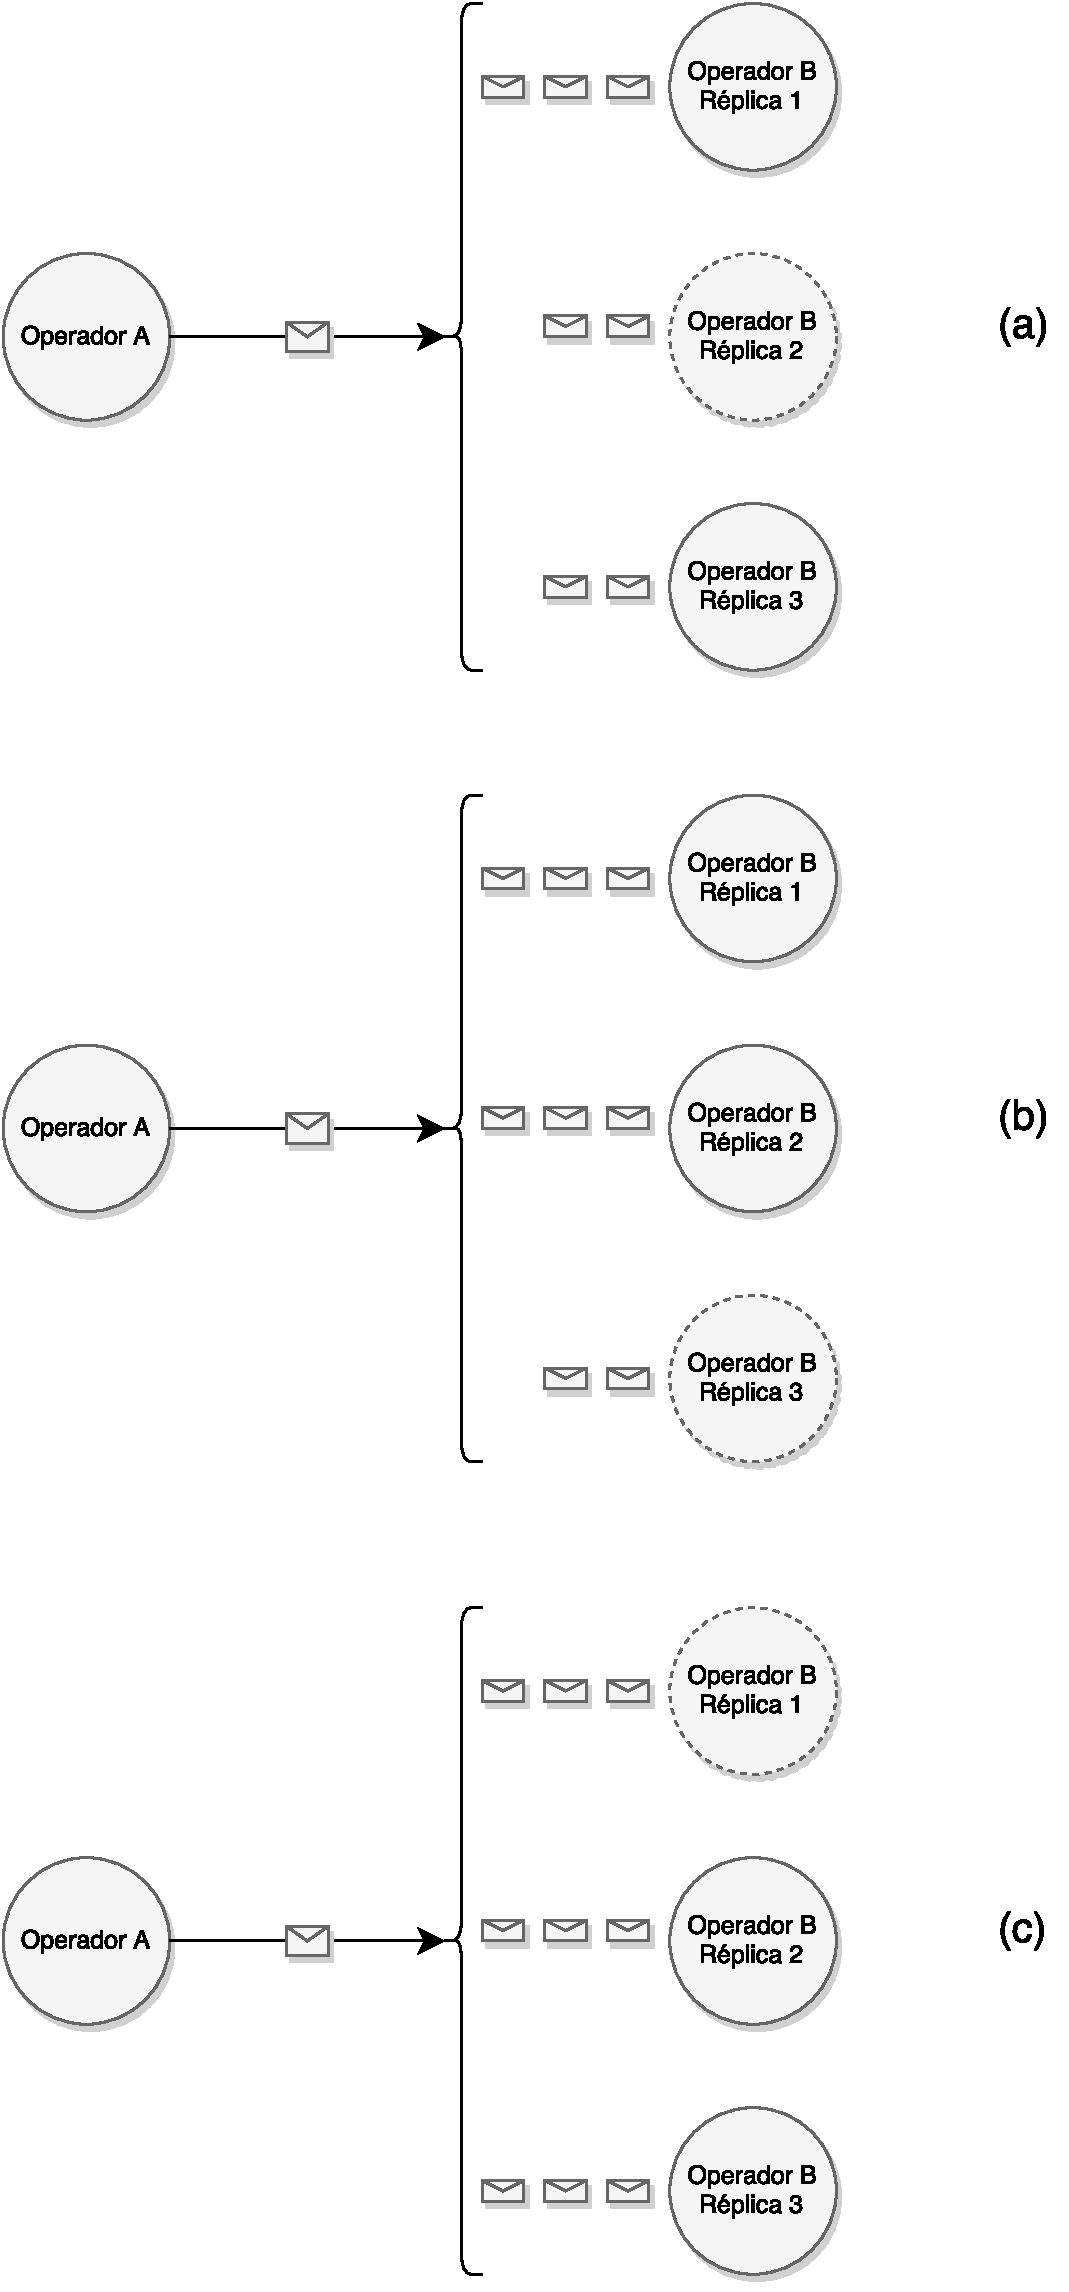
\includegraphics[scale=0.45]{images/DistribucionCarga.pdf}
	\caption{Distribución de la carga entre las réplicas.}
	\label{fig:distCarga}
\end{figure}

En el Algoritmo \ref{alg:distCarga} está descrito la distribución de carga planteada anteriormente, la cual fue implementada en S4 para realizar los experimentos según lo diseñado en el planteamiento de los algoritmos.

\begin{algorithm}[!ht]
	\caption{Distribución de carga entre las réplicas de un operador.}
	\label{alg:distCarga}
	\begin{algorithmic}[1]
	\REQUIRE Evento $\epsilon$ y operador $\phi$.
	\ENSURE Envío del evento a la réplica disponible del operador $\phi$.
	\STATE $\theta \leftarrow minTamanoCola(\phi)$ \COMMENT Se escoge la réplica que posea menor cola
	\STATE $envioEvento(\epsilon,\theta$)
	\end{algorithmic}
\end{algorithm}

\section{Diseño de los experimentos}
Para los experimentos se diseñaron tres aplicaciones, una que realiza operaciones con estado, otra que no, y otra sintética. En el caso que la aplicación posea estado, significa que el operador guarda variables con el transcurso del tiempo, las cuales van a ser entregadas cada cierto tiempo o al finalizar la ejecución del sistema. Este tipo de aplicaciones son las más utilizadas, dado que utilizan contadores o variables globales, las cuales son necesarias para el análisis de los datos. Un ejemplo de esto, es un sistema que cuenta las palabras de un texto y que envié la cantidad de palabras contadas cada cierta ventana de tiempo. Si bien, las aplicaciones sin estado no son tan utilizadas, se consideraron importantes para la validación del modelo, dado que son las aplicaciones más simples y básicas de diseñar y ejecutar. Por otra parte, la aplicación sintética se refiere a un sistema cuyos operadores sólo generan tiempo de demora artificial, en el caso de este experimento, se dejo durmiendo la hebra asignada al operador un período determinado de tiempo.

Para la generación del \textit{stream} de la fuente de datos para la primera y segunda aplicación, se utilizó 4.5 millones de \textit{tweets}, los cuales fueron recolectados entre los días 27-28 de Febrero y 1-2 de Marzo de 2010, tanto en inglés, portugués y español. Estos contenían información correspondiente a la interacción entre los usuarios debido al terremoto ocurrido el 27 de Febrero en Chile.

Por otra parte, el envío de los datos anteriores se realizó de dos maneras: constante y variable. La primera forma consiste en enviar 100 eventos por segundo constantemente. En cambio, la segunda forma consiste en enviar 50 eventos por segundos el primer tercio del experimento, para luego aumentar a a 100 eventos por segundo en el segundo tercio, y finalmente, disminuir a 50 eventos por segundos el último tercio de la ejecución.

\subsection{Aplicación 1: Análisis de \textit{tweets} en escenarios de desastres naturales}
La primera aplicación fue orientada a un caso de desastres naturales, donde se generó un grafo que pudiera realizar un filtrado de palabras y análisis de los datos. Ninguno de los operadores posee estado, por lo tanto son independientes. Para la duración de esta prueba se consideró un tiempo de 70 minutos. El objetivo de esta aplicación, era comprobar que el sistema diseñado puede funcionar con aplicaciones sin estados, las cuales son las más básicas y sencillas de diseñar en SPS, y que tienen utilidad cuando se hacen análisis directo del flujo de datos.

La aplicación consta del flujo de datos, cuyos datos serán la muestra de \textit{tweets} de prueba, y cuatro operadores, los cual son denominados \textit{Stopword}, \textit{Language}, \textit{Counter} y \textit{MongoDB}.

\paragraph{Stopword:} está encargado de analizar el \textit{tweet} y remover las palabras no relevantes para el análisis de éste, basado en una bolsa de palabras, cuyas palabras se llaman \textit{stopwords}. De esta manera, se puede analizar el texto usando las palabras más representativas de éste y así entregar información más precisa.

\paragraph{Language:} está encargado de analizar el lenguaje existente en el \textit{tweet}, para esto se utilizó una librería \textit{Apache Tika} \citep{mattmann2011tika}. Con ésta se puede realizar un filtro del idioma de los tweets, de tal manera que en caso de ser requerido, sólo continúen los de un idioma en específico, en nuestro caso el español.

\paragraph{Counter:} está encargado de contar e indicar la cantidad de palabras que existen en el \textit{tweet} según una bolsa de palabras proporcionada por el programador. Para esta prueba se utilizó una bolsa de 26.000 palabras en español. Con esto se podría realizar un análisis de los \textit{tweets} que poseían mayor cantidad de palabras claves asociados a una temática o evento en particular.

\paragraph{MongoDB:} está encargado de guardar en la base de datos el evento según los atributos que éste posea, ya sea por el \textit{tweet} original, sin \textit{stopword}, idioma y cantidad de palabras claves existentes en él. Para esto, se utilizó el motor de base de datos no relacional \textit{MongoDB} \citep{chodorow2013mongodb}.

En la Figura \ref{fig:primeraAplicacion} se muestra un ejemplo de la aplicación con sus distintos operadores y relaciones. Las flechas muestran la dirección del flujo de datos emitido por la fuente y los operadores.

\begin{figure}[!hb]
	\centering
		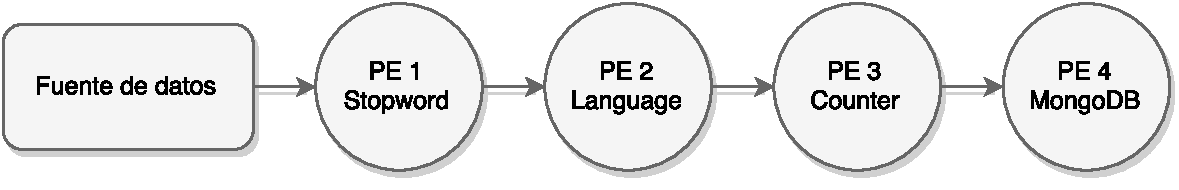
\includegraphics[scale=0.75]{images/App1.pdf}
	\caption{Aplicación 1.}
	\label{fig:primeraAplicacion}
\end{figure}

\subsection{Aplicación 2: Contador de palabras en muestras de textos}
La segunda aplicación consiste en un contador de palabras, el cual cuenta la cantidad de veces que se repite una palabra en un conjunto de datos según una bolsa de palabras establecida por el usuario. Esta aplicación se considera con estado, debido que debe existir un contador en el operador, de tal manera de contar la cantidad de veces que se repite cierta palabra de la bolsa de palabras en los datos entrantes. Con esta aplicación es posible analizar posteriormente las palabras más frecuentes emitidas por los usuarios de la red social según un listado de palabras claves. Para la duración de esta prueba se consideró un tiempo de 70 minutos. El objetivo de esta aplicación era validar el sistema diseñado con aplicaciones con estado, las cuales son las más aplicadas, debido que se realizan análisis generales de los datos, como el caso de los \textit{trending topics} o frecuencia de palabras.

La aplicación consta del flujo de datos, cuyos datos serán la muestra de \textit{tweets} de prueba, y tres operadores, denominados \textit{Split}, \textit{Counter} y \textit{Merge}.

\paragraph{Split:} está encargado de dividir el \textit{tweet}, y enviar un arreglo con las palabras que poseía este texto al operador \textit{Counter}.

\paragraph{Counter:} está encargado de guardar las estadísticas de los contadores de cada palabra, es decir, en el momento que reciba un evento, este analiza las palabras que posee y aumenta el contar de la palabra en el operador. Las estadísticas son enviadas cada 10 segundos al operador Merge, de tal manera de no enviar flujo constante al siguiente operador y generar mayor cantidad de carga.

\paragraph{Merge:} está encargado de unir las distintas estadísticas enviadas por las distintas réplicas del operador Counter.

En la Figura \ref{fig:segundaAplicacion} se muestra un ejemplo de la segunda aplicación con sus distintos operadores y sus relaciones, de igual manera que en el caso anterior, las flechas reflejan el flujo de datos. Cabe destacar que el único operador que puede replicarse es el \textit{Counter}, debido que el operador \textit{Split} y \textit{Merge} son operadores que soportan la replicación del operador \textit{Counter}, como se explicó en las técnicas de balance de carga en la subsección \ref{sec:fisionBC}.

\begin{figure}[!ht]
	\centering
		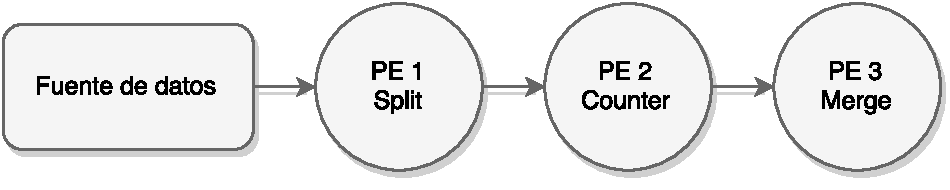
\includegraphics[scale=0.75]{images/App2.pdf}
	\caption{Aplicación 2.}
	\label{fig:segundaAplicacion}
\end{figure}

\subsection{Aplicación 3: Aplicación sintética}
La tercera aplicación consta de tres operadores, los cuales duermen a la hebra asignada al operador un determinado período de tiempo. De esta manera, se genera un tiempo de espera artificial, realizando un operador sintético, de tal manera que pueda simular el comportamiento de un operador real. El objetivo de realizar este tipo de aplicación, fue analizar los costos que poseía el sistema implementando para la optimización del sistema.

La Tabla \ref{tab:app3-time} muestra el período de tiempo que duerme cada PEs a su hebra asignada. Los tiempos que se consideraron para esta prueba es para generar una sobrecarga en el primer y segundo operador, de tal manera que después afectarán al tercer operador. Para la duración de esta prueba se consideró un tiempo de 15 minutos.

\begin{table}[!ht]
\centering
\caption{Período de tiempo que duerme la hebra asignada al PE.}
\begin{tabular}{| c | c |}
\hline
PE & Tiempo (ms) \\ \hline
1 & 20 \\
2 & 30 \\
3 & 15 \\\hline
\end{tabular}
\label{tab:app3-time}
\end{table}

En la Figura \ref{fig:terceraAplicacion} se muestra un ejemplo de la tercera aplicación con sus distintos operadores y sus relaciones, de igual manera que en los casos anteriores, las flechas reflejan el flujo de datos.

\begin{figure}[!hb]
	\centering
		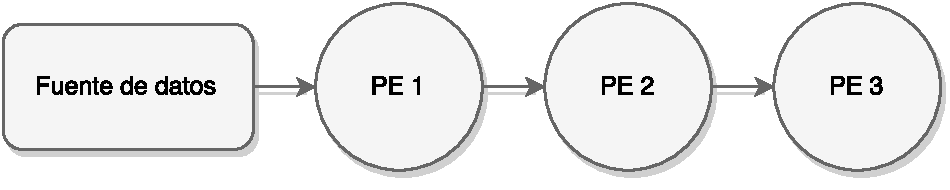
\includegraphics[scale=0.75]{images/App3.pdf}
	\caption{Aplicación 3.}
	\label{fig:terceraAplicacion}
\end{figure}

\section{Evaluación}

Para la ejecución de los experimentos, se utilizó un servidor con sistema operativo Ubuntu 14.04.2 LTS, cuyo procesador es un Intel\textregistered Xeon\textregistered CPU E5-2650 v2 de 2.60GHz y con 32 GB de RAM. Cabe recalcar, que el lenguaje de programación fue Java, debido a la integración del sistema propuesto en el SPS utilizado, el cual fue S4. La configuración de la configuración de S4 está detallada en el Anexo \ref{apendice:config-comm-S4}.

La recolección de estadísticas fue realizada cada 5 segundos, por lo que desde ahora se hablará período un intervalo de tiempo de 5 segundos entre cada recolección de las estadísticas.

\subsection{Aplicación 1: Análisis de \textit{tweets} en escenarios de desastres naturales}
En la primera aplicación se procedió a realizar dos experimentos, donde el primero consta un envío constante de datos, y el segundo un envío variable. En ambos experimentos, se consideraron dos pruebas, donde la primera consistía en la ejecución de la aplicación en un sistema SPS que use el sistema de distribución de carga, y la segunda sin uso de éste, por lo que cada par de figuras son la comparación de la aplicación con y sin monitor respectivamente.

Para el análisis de los experimentos, se consideró la cantidad promedio de eventos procesados en un período, la cantidad total de eventos procesados y las estadísticas de cada PE en el transcurso de la ejecución de la aplicación.

En el primer experimento se puede ver que en las Figuras \ref{fig:app1-uniform-statusStopwordPE-cm} y \ref{fig:app1-uniform-statusStopwordPE-sm}, se muestran las estadísticas del primer operador del grafo, con y sin monitoreo en la carga de los operadores respectivamente, ambas con un envío constante de la fuente de datos. Se puede observar que en el primer gráfico se presenta una tasa de llegada ($\lambda$) constante, a diferencia del segundo gráfico, donde en el segundo 2600 presenta una variación.

Lo anterior se debe a la acumulación de eventos en el \textit{buffer} del operador, por lo que al llenarse éste, bloquea la recepción de eventos al operador. De esta manera, se debe esperar que se liberen eventos del \textit{buffer}, pero como la tasa de rendimiento es baja, al desencolarse, inmediatamente llegada otro evento que vuelve a llenarlo, por lo que la cola se mantiene constante después del segundo 2600. Es por esto, que la tasa de llegada disminuye aproximadamente al mismo valor de la tasa de procesamiento.

Por otra parte, la tasa de rendimiento ($\rho$) de la Figura \ref{fig:app1-uniform-statusStopwordPE-cm} se estabiliza dentro de los primeros 100 segundos, debido que el sistema de distribución de carga detecta el operador sobrecargado y lo replica, a diferencia de la Figura \ref{fig:app1-uniform-statusStopwordPE-sm}, en el cual el operador posee una tasa de rendimiento inestable que fluctúa entre 1 y 2, hasta el segundo 2600, donde disminuye debido que la tasa de llegada es menor. Cabe destacar que este operador posee un alto costo computacional, debido que existe una gran cantidad de palabras que debe analizar con cada una de las palabras del texto, por lo que es necesario crear otra réplica debido a la sobrecarga existente.

En las Figuras \ref{fig:app1-uniform-statusLanguagePE-cm} y \ref{fig:app1-uniform-statusLanguagePE-sm} se puede ver el siguiente operador del gráfico, el cual no tiene mayor inconveniente, a excepción del segundo 2400, donde el caso sin monitoreo disminuye considerablemente la tasa de procesamiento del PE. Si analizamos las Figuras \ref{fig:app1-uniform-statusStopwordPE-sm} y \ref{fig:app1-uniform-statusLanguagePE-sm}, empiezan aproximadamente desde el rango de tiempo (2400s, 2600s) los problemas de procesamiento de los operadores, por lo tanto, se puede deducir que si el problema surge en un operador no es un problema aislado, sino que también influye a los siguientes operadores.

Se puede observar como con el transcurso de los primeros 100 segundos en la Figura \ref{fig:app1-uniform-statusCounterPE-cm}, fue aumentando la cantidad de réplicas hasta llegar a 5, el cual fue su óptimo, para ir procesando la cantidad de eventos y disminuir la cola existente en el sistema. Esto en contra posición a la Figura \ref{fig:app1-uniform-statusCounterPE-sm}, donde la inexistencia de replicación, genera una cola la cual se mantiene constante en el segundo 2400.

Finalmente, se encuentra el último operador, el cual no presenta grandes inconvenientes tanto en las Figuras \ref{fig:app1-uniform-statusMongoPE-cm} y \ref{fig:app1-uniform-statusMongoPE-sm}, esto debido que el tiempo de procesamiento es bajo, y nunca llega una cantidad de eventos considerable para existir una sobrecarga en éste. Además es importante destacar que en la Figura \ref{fig:app1-uniform-statusMongoPE-sm} se registra una menor tasa de llegada, con un promedio de $83\%$ menos de eventos que un SPS ejecutado con el sistema de distribución de carga.

Por otra parte, también se analizó la cantidad promedio de eventos procesados en cada período, la cual está graficada en las Figuras \ref{fig:app1-uniform-cm-avgEventProcess} y \ref{fig:app1-uniform-sm-avgEventProcess}. Como se puede apreciar, en los primeros 50 segundos se puede ver una mejora considerable en la cantidad de eventos procesados, donde posteriormente se procesan aproximadamente 480 eventos por período con monitoreo, a diferencia del SPS sin monitoreo, que procesa 90 eventos por período aproximadamente, procesándose 5 veces más eventos. Esta mejora se debe al factor de la replicación de los operadores que posee mayor sobrecarga, por lo que al aumentar la cantidad de réplicas, aumenta la tasa de procesamiento, lo significa mayor cantidad de flujo para el próximo operador.

Así también, se puede observar en las Figuras \ref{fig:app1-uniform-eventCount-cm} y \ref{fig:app1-uniform-eventCount-sm} la cantidad total de eventos procesados con el transcurso de la ejecución en cada uno de los operadores, con y sin uso del monitoreo respectivamente. En el primer gráfico se denota como los cuatro operadores del SPS van aumentando linealmente con la misma pendiente, tan sólo existe una menor cantidad de eventos procesados en el tercer PE, lo cual se traslada al cuatro PE, debido que al procesar menor cantidad de eventos el tercer PE, llega menor cantidad de datos al cuarto PE. En este gráfico se llegó a un total de 401.618 eventos procesados. En cambio, en el segundo gráfico existen pendientes muy distintas por los distintos operadores, lo cual se ve reflejado desde la cantidad de eventos procesados en el primer operador hasta la cantidad total de eventos procesados por el sistema, el cual es de 67.141, procesando 6 veces más eventos en el mismo período de tiempo la aplicación con el uso del sistema de monitoreo.

\begin{figure}[p]
\centering
    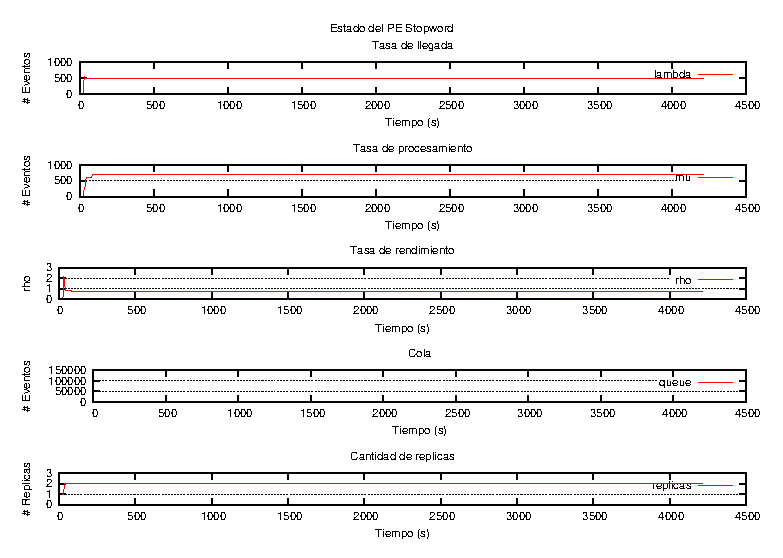
\includegraphics[scale=1.1]{images/exp/app1/uniform/cm/statusStopwordPE.eps}
    \caption{Estadísticas del PE Stopword en la primera aplicación con un envío constante de la fuente de datos con uso del monitor.}
    \label{fig:app1-uniform-statusStopwordPE-cm}
\end{figure}

\begin{figure}[p]
\centering
    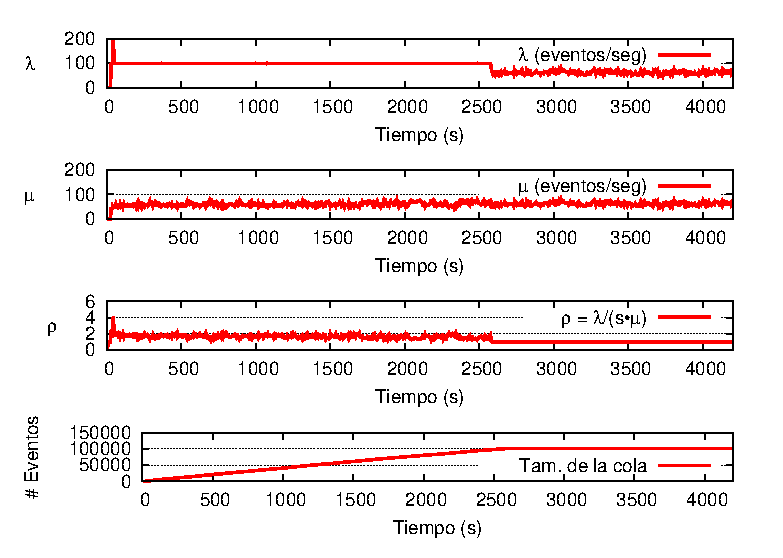
\includegraphics[scale=1.1]{images/exp/app1/uniform/sm/statusStopwordPE.eps}
    \caption{Estadísticas del PE Stopword en la primera aplicación con un envío constante de la fuente de datos sin uso del monitor.}
    \label{fig:app1-uniform-statusStopwordPE-sm}
\end{figure}

\begin{figure}[p]
\centering
    \includegraphics[scale=1.1]{images/exp/app1/uniform/cm/statusLanguagePE.eps}
    \caption{Estadísticas del PE Language en la primera aplicación con un envío constante de la fuente de datos con uso del monitor.}
    \label{fig:app1-uniform-statusLanguagePE-cm}
\end{figure}

\begin{figure}[p]
\centering
    \includegraphics[scale=1.1]{images/exp/app1/uniform/sm/statusLanguagePE.eps}
    \caption{Estadísticas del PE Language en la primera aplicación con un envío constante de la fuente de datos sin uso del monitor.}
    \label{fig:app1-uniform-statusLanguagePE-sm}
\end{figure}

\begin{figure}[p]
\centering
    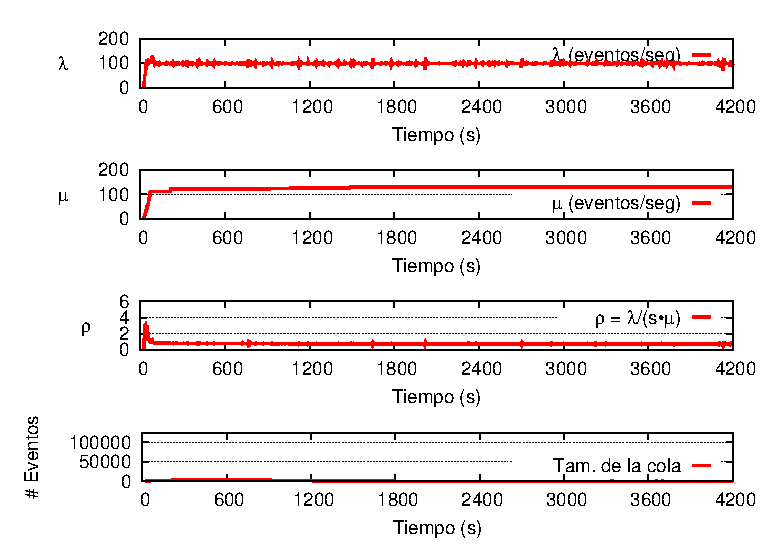
\includegraphics[scale=1.1]{images/exp/app1/uniform/cm/statusCounterPE.eps}
    \caption{Estadísticas del PE Counter en la primera aplicación con un envío constante de la fuente de datos con uso del monitor.}
    \label{fig:app1-uniform-statusCounterPE-cm}
\end{figure}

\begin{figure}[p]
\centering
    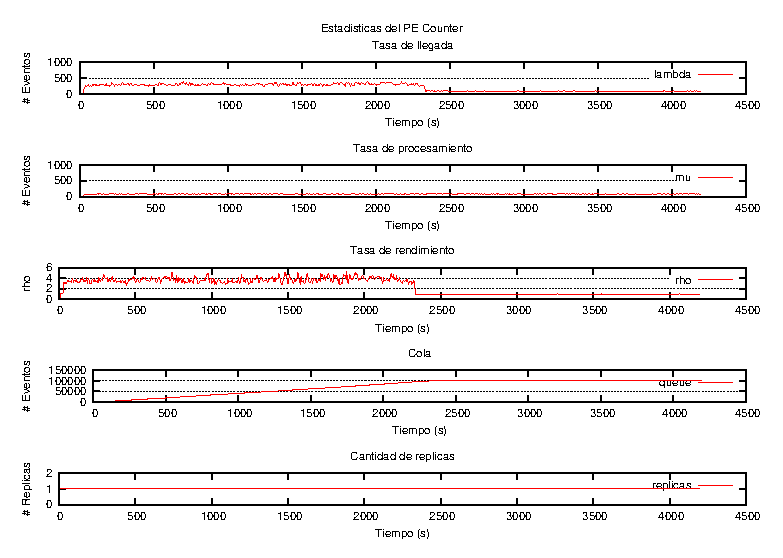
\includegraphics[scale=1.1]{images/exp/app1/uniform/sm/statusCounterPE.eps}
    \caption{Estadísticas del PE Counter en la primera aplicación con un envío constante de la fuente de datos sin uso del monitor.}
    \label{fig:app1-uniform-statusCounterPE-sm}
\end{figure}

\begin{figure}[p]
\centering
    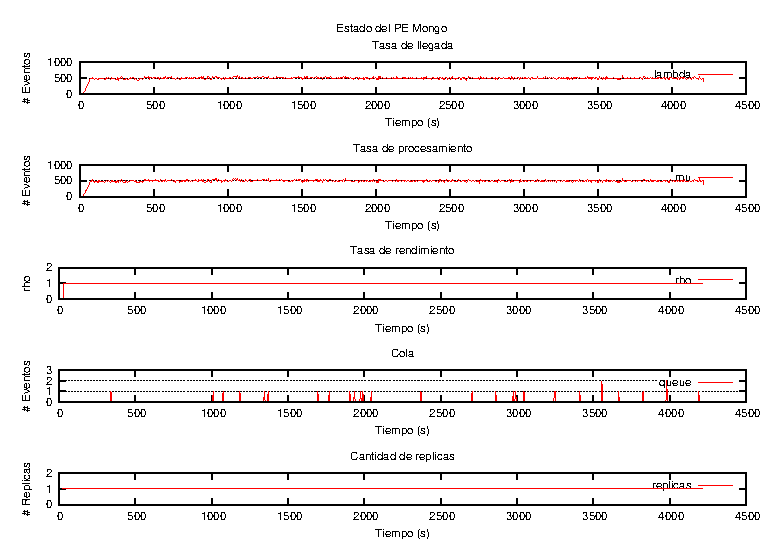
\includegraphics[scale=1.1]{images/exp/app1/uniform/cm/statusMongoPE.eps}
    \caption{Estadísticas del PE Mongo en la primera aplicación con un envío constante de la fuente de datos con uso del monitor.}
    \label{fig:app1-uniform-statusMongoPE-cm}
\end{figure}

\begin{figure}[p]
\centering
    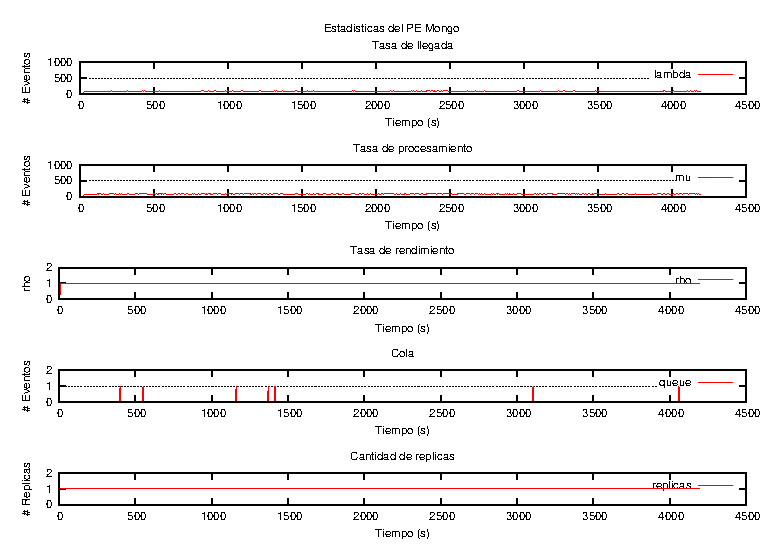
\includegraphics[scale=1.1]{images/exp/app1/uniform/sm/statusMongoPE.eps}
    \caption{Estadísticas del PE Mongo en la primera aplicación con un envío constante de la fuente de datos sin uso del monitor.}
    \label{fig:app1-uniform-statusMongoPE-sm}
\end{figure}

\begin{figure}[ht]
\centering

\begin{minipage}[c]{0.45\textwidth}
\centering
    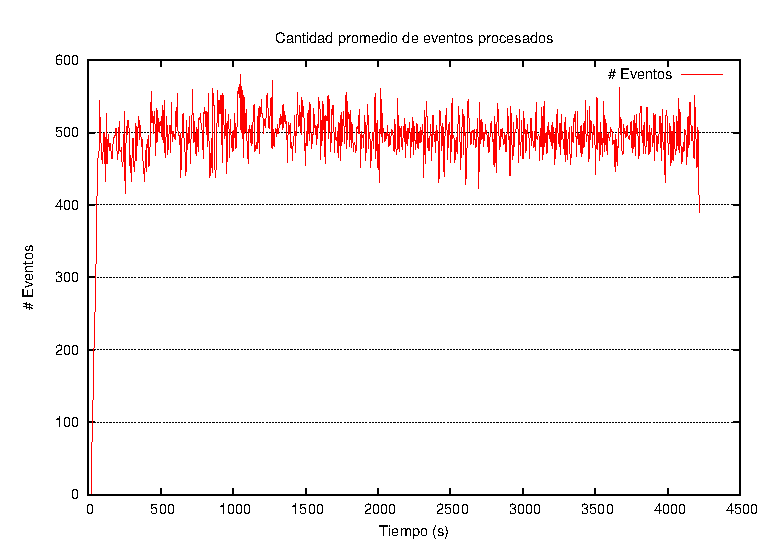
\includegraphics[width=\textwidth]{images/exp/app1/uniform/cm/avgEventProcess.eps}
    \caption{Tiempo promedio de procesamiento de un evento en la primera aplicación con un envío constante de la fuente de datos usando monitor.}
    \label{fig:app1-uniform-cm-avgEventProcess}
\end{minipage} \hspace*{1cm}
\begin{minipage}[c]{0.45\textwidth}
\centering
    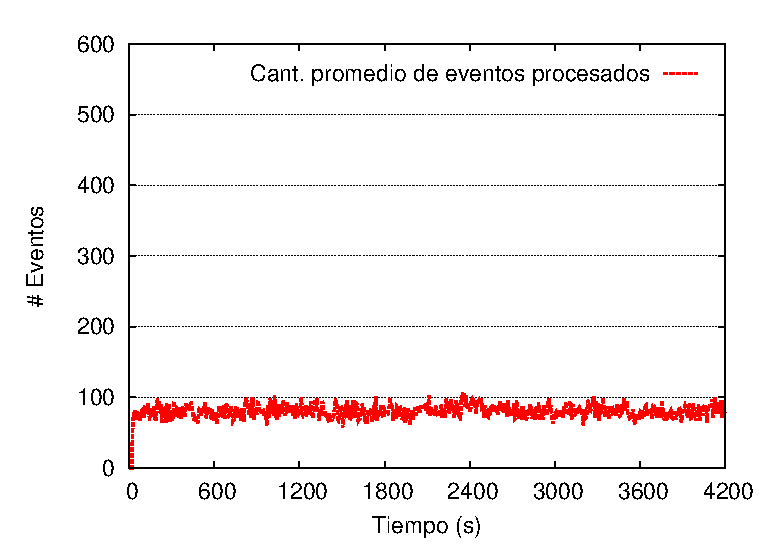
\includegraphics[width=\textwidth]{images/exp/app1/uniform/sm/avgEventProcess.eps}
    \caption{Tiempo promedio de procesamiento de un evento en la primera aplicación con un envío constante de la fuente de datos no usando monitor.}
    \label{fig:app1-uniform-sm-avgEventProcess}
\end{minipage}

\end{figure}

\begin{figure}[ht]
\centering

\begin{minipage}[c]{0.45\textwidth}
\centering
    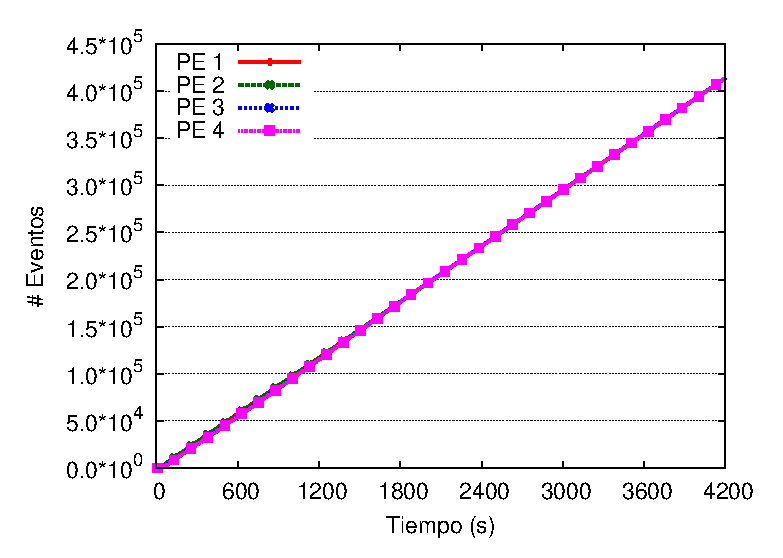
\includegraphics[width=\textwidth]{images/exp/app1/uniform/cm/eventCount.eps}
    \caption{Cantidad total de eventos procesados en la primera aplicación con un envío constante de la fuente de datos usando monitor.}
    \label{fig:app1-uniform-eventCount-cm}
\end{minipage} \hspace*{1cm}
\begin{minipage}[c]{0.45\textwidth}
\centering
    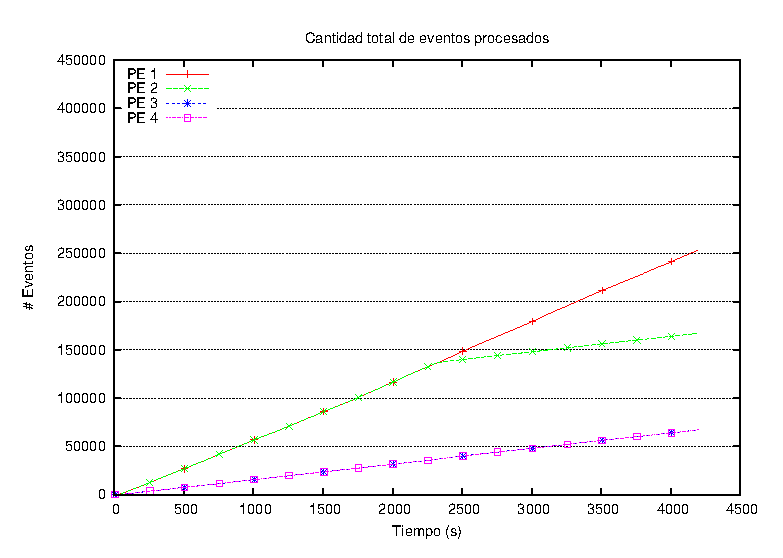
\includegraphics[width=\textwidth]{images/exp/app1/uniform/sm/eventCount.eps}
    \caption{Cantidad total de eventos procesados en la primera aplicación con un envío constante de la fuente de datos no usando monitor.}
    \label{fig:app1-uniform-eventCount-sm}
\end{minipage}

\end{figure}

En el segundo experimento se puede apreciar que en las Figuras \ref{fig:app1-normal-statusStopwordPE-cm} y \ref{fig:app1-normal-statusStopwordPE-sm}, se muestra el comportamiento del primer operador con un envío variable de la fuente de datos. En las estadísticas se observa que existe un comportamiento estable hasta el segundo 1100, con y sin uso del monitor. Esto se debe a que el operador no posee gran cantidad de demanda dada la tasa de llegada, el cual varía en el segundo 1100, debido que aumenta la cantidad de eventos entrantes. Debido a esto es que el operador debe procesar mayor cantidad de datos, aumentando así la cantidad de réplicas del operador. Luego en el segundo 3200 disminuye la tasa de llegada, por lo que la tasa de rendimiento vuelve a ser estable en el sistema con y sin monitoreo, debido a que es menor la cantidad de eventos que deben ser procesados, lo que significa también la disminución de una réplica en el sistema con uso del monitoreo.

El comportamiento variable del flujo de entrada sólo se puede apreciar con mayor detalle en el primer operador cuando no se utiliza monitor, debido que la tasa de llegada del segundo depende de la tasa de procesamiento del primero, y cómo no existe un aumento de la tasa de procesamiento, sólo aumenta hasta lo que pueda procesar con un sólo operador. En las Figuras \ref{fig:app1-normal-statusLanguagePE-cm} y \ref{fig:app1-normal-statusLanguagePE-sm} se puede apreciar la diferencia entre las tasas de llegada, debido que en el primer gráfico, existe una variación de la tasa de llegada, debido al uso del sistema de monitoreo, a diferencia del segundo gráfico. Esto se debe a que el primer operador no procesa todos los eventos entrantes, significa que la tasa de llegada sea constante en el segundo operador. Independiente del uso o no del monitor, no existe una sobrecarga en el operador, por lo que el comportamiento siempre es estable del operador.

Luego, en las Figuras \ref{fig:app1-normal-statusCounterPE-cm} y \ref{fig:app1-normal-statusCounterPE-sm} se presenta el tercer operador, el cual existe una sobrecarga desde el inicio del sistema. Esto se debe a la gran cantidad de palabras que debe comparar, por lo que al realizar la iteración para verificar si existe o no una palabra, requiere un alto costo computacional. En el primer gráfico se puede analizar que en los primeros 100 segundos, aumenta a tres réplicas, estabilizándose el rendimiento del operador. En cambio, en el sistema sin monitoreo existe una tasa de servicio es constante, por lo que la tasa de rendimiento es inestable en el transcurso de todo el experimento. También se muestra una disminución en la cantidad de réplicas en el segundo 3200, y esto se debe que la cantidad de réplicas necesarias para el sistema son menos, dado que el envío de datos de la fuente de datos disminuyó, por lo que la tasa de llegada del PE también.

Dentro de los análisis importantes que se pueden realizar al gráfico, es que en el primer tercio de la prueba con uso del monitor, la cantidad óptima de operadores fue 4, pero en el último tercio fue de 5, siendo que ambos poseen la misma tasa de llegada. Esto se debe a que al aumentar a 7 réplicas en el segundo tercio, al disminuir la tasa de llegada en el último tercio, se detectó que los operadores se encontraban ociosos, por lo que era necesario remover réplicas. Esto se debe a su $\rho$ es menor a 0.5, por lo tanto para encontrarse a un estado estable, es necesario converger a 0.5, por lo que al estabilizarse el operador, su $\rho$ tiende a estar más cerca de 0.5 que de 1. De esta manera, las tasas de rendimiento son distintas en el primer y último tercio, por lo que puede darse que las réplicas del primer tercio sea mayor que el último tercio.

Por último, en el cuarto operador se puede apreciar en las Figuras \ref{fig:app1-normal-statusMongoPE-cm} y \ref{fig:app1-normal-statusMongoPE-sm} el comportamiento con y sin monitoreo. En ambos casos se muestra una tasa de rendimiento estable, la diferencia está en la tasa de llegada que posee cada uno de los sistemas, donde en el primer gráfico la tasa de llegada es variable, y en el segundo es constante, por lo que existe una menor tasa de servicio, lo que significa que la cantidad de datos procesados es menor.

Como se ha expuesto anteriormente, la cantidad de datos procesados en el sistema sin monitoreo es menor, y esto se puede apreciar en la cantidad promedio de eventos procesados en cada período como se muestra en las Figuras \ref{fig:app1-normal-cm-avgEventProcess} y \ref{fig:app1-normal-sm-avgEventProcess}. En el primer gráfico existe un promedio de 225 eventos por período, el cual aumenta a un promedio de 438 eventos por período en el segundo 1100, debido que el flujo de la fuente de datos aumenta, para que luego disminuya a un promedio de 332 eventos por período en el segundo 3200 debido a la disminución de la tasa de llegada. En cambio, en el segundo gráfico la cantidad promedio de eventos procesados es constante, debido que no existe optimización alguna en el sistema, por lo que en todo el experimento se procesan 98 eventos por período aproximadamente. Dado esto, en el primer tramo existe una mejora de 2 veces más eventos, luego en el segundo tramo una mejora de 4 veces más, y por último, tercer tramo una mejora de 3 veces más.

Finalmente, la cantidad total de eventos procesados en cada experimento, se puede ver en las Figuras \ref{fig:app1-normal-eventCount-cm} y \ref{fig:app1-normal-eventCount-sm}. En el primer gráfico se puede ver dos variaciones de la curva, en el segundo 1100 y 3200, lo cual son los segundos en los cuales hubo una variación en el flujo de la fuente de datos, por lo que aumenta y disminuye respectivamente en esos segundos la tasa de llegada del sistema. En cambio, en el segundo gráfico no se denota esto, debido que independiente de la tasa de llegada, el procesamiento del sistema siempre es constante, debido que no se adapta a la carga que posea cada operador con el transcurso del tiempo. El sistema con uso del monitor procesa un total de $303.156$, contra $82.770$ eventos en total sin uso del monitor, lo cual significa un aumento del 3 veces más eventos procesados.

\begin{figure}[p]
\centering
    \includegraphics[scale=1.1]{images/exp/app1/normal/cm/statusStopwordPE.eps}
    \caption{Estadísticas del PE Stopword en la primera aplicación con un envío variable de la fuente de datos con uso del monitor.}
    \label{fig:app1-normal-statusStopwordPE-cm}
\end{figure}

\begin{figure}[p]
\centering
    \includegraphics[scale=1.1]{images/exp/app1/normal/sm/statusStopwordPE.eps}
    \caption{Estadísticas del PE Stopword en la primera aplicación con un envío variable de la fuente de datos sin uso del monitor.}
    \label{fig:app1-normal-statusStopwordPE-sm}
\end{figure}

\begin{figure}[p]
\centering
    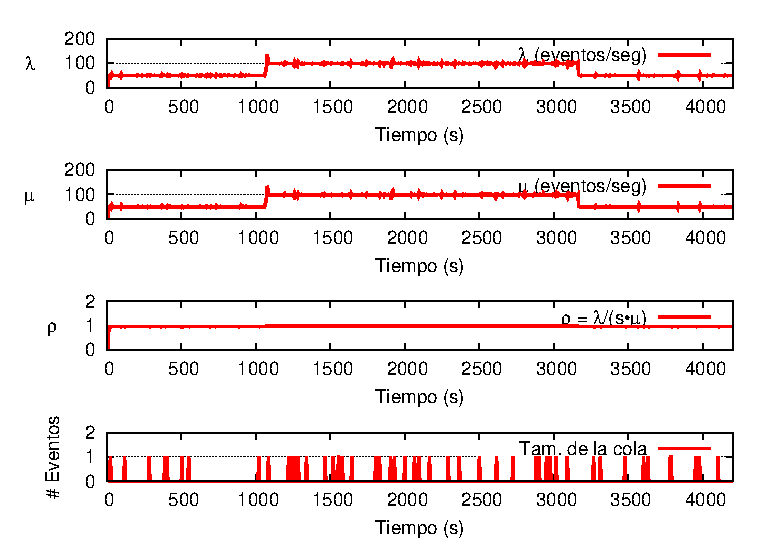
\includegraphics[scale=1.1]{images/exp/app1/normal/cm/statusLanguagePE.eps}
    \caption{Estadísticas del PE Language en la primera aplicación con un envío variable de la fuente de datos con uso del monitor.}
    \label{fig:app1-normal-statusLanguagePE-cm}
\end{figure}

\begin{figure}[p]
\centering
    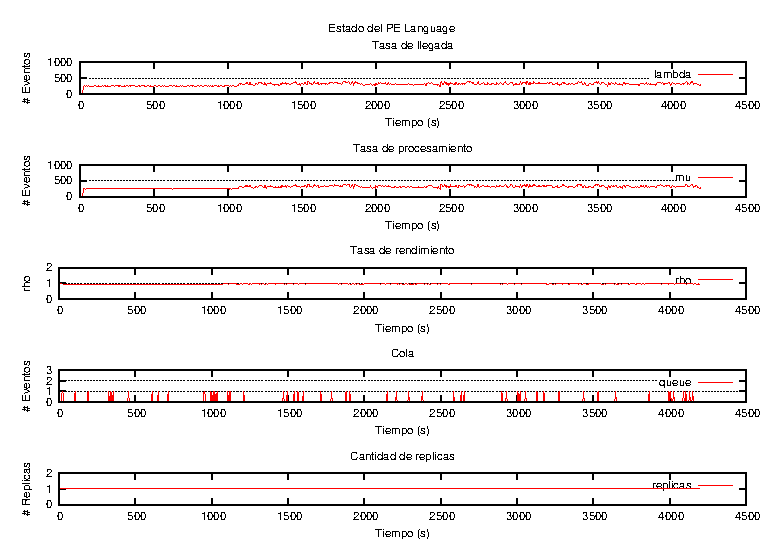
\includegraphics[scale=1.1]{images/exp/app1/normal/sm/statusLanguagePE.eps}
    \caption{Estadísticas del PE Language en la primera aplicación con un envío variable de la fuente de datos sin uso del monitor.}
    \label{fig:app1-normal-statusLanguagePE-sm}
\end{figure}

\begin{figure}[p]
\centering
    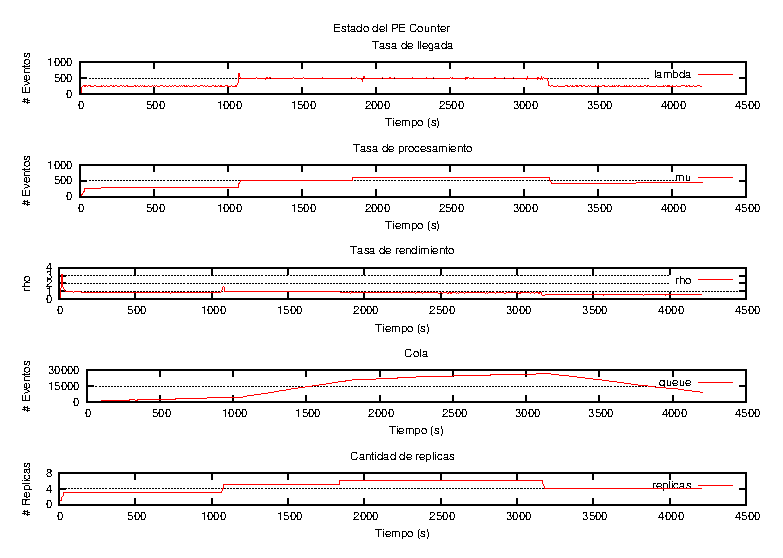
\includegraphics[scale=1.1]{images/exp/app1/normal/cm/statusCounterPE.eps}
    \caption{Estadísticas del PE Counter en la primera aplicación con un envío variable de la fuente de datos con uso del monitor.}
    \label{fig:app1-normal-statusCounterPE-cm}
\end{figure}

\begin{figure}[p]
\centering
    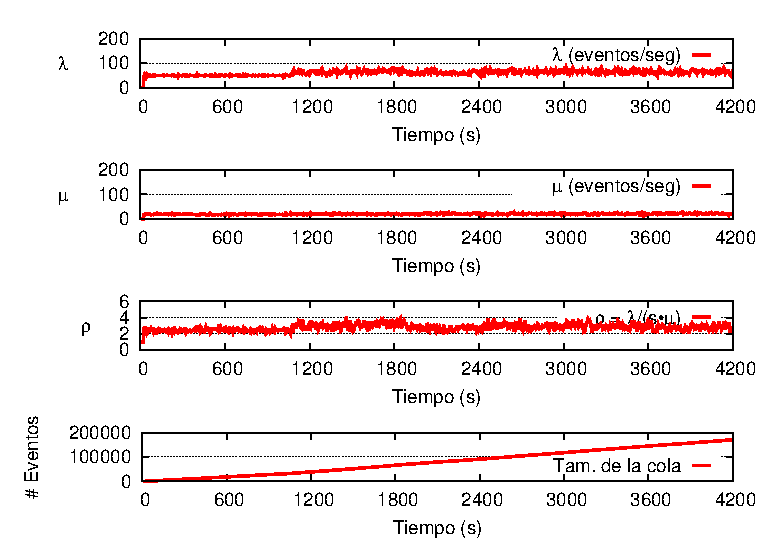
\includegraphics[scale=1.1]{images/exp/app1/normal/sm/statusCounterPE.eps}
    \caption{Estadísticas del PE Counter en la primera aplicación con un envío variable de la fuente de datos sin uso del monitor.}
    \label{fig:app1-normal-statusCounterPE-sm}
\end{figure}

\begin{figure}[p]
\centering
    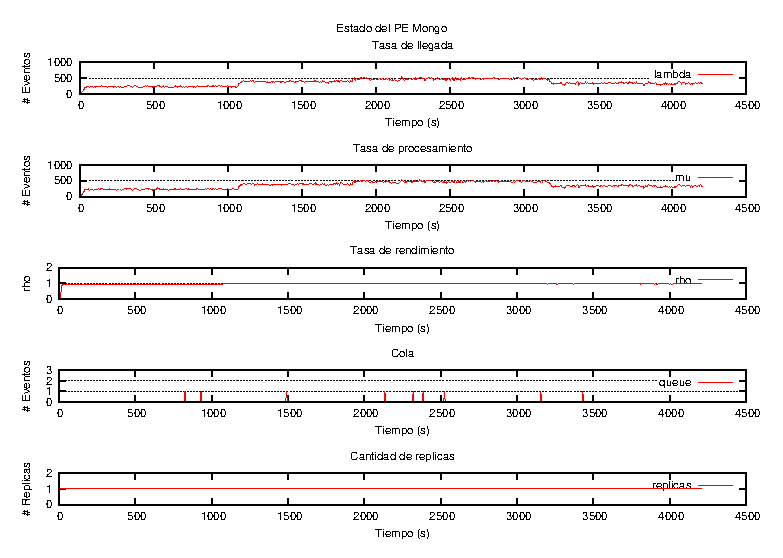
\includegraphics[scale=1.1]{images/exp/app1/normal/cm/statusMongoPE.eps}
    \caption{Estadísticas del PE Mongo en la primera aplicación con un envío variable de la fuente de datos con uso del monitor.}
    \label{fig:app1-normal-statusMongoPE-cm}
\end{figure}

\begin{figure}[p]
\centering
    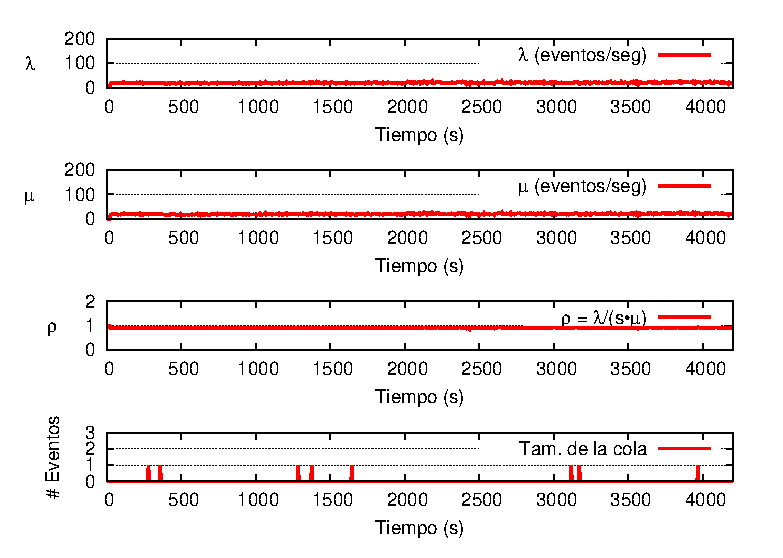
\includegraphics[scale=1.1]{images/exp/app1/normal/sm/statusMongoPE.eps}
    \caption{Estadísticas del PE Mongo en la primera aplicación con un envío variable de la fuente de datos sin uso del monitor.}
    \label{fig:app1-normal-statusMongoPE-sm}
\end{figure}

\begin{figure}[!ht]
\centering

\begin{minipage}[c]{0.45\textwidth}
\centering
    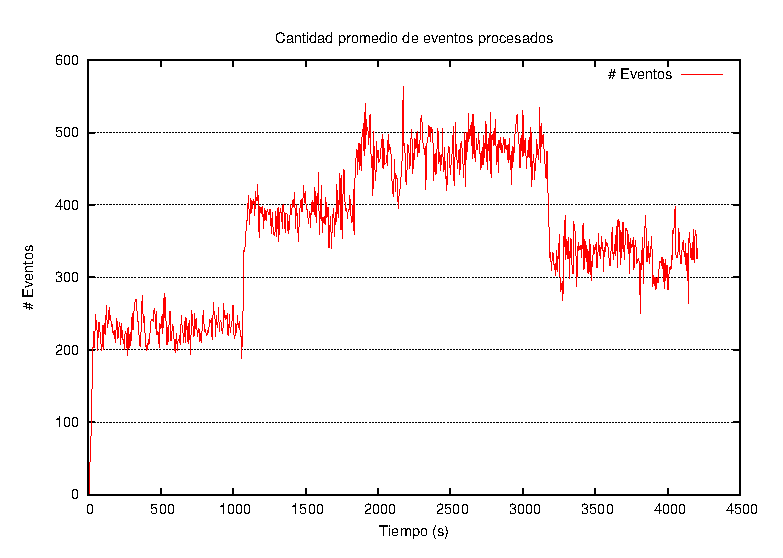
\includegraphics[width=\textwidth]{images/exp/app1/normal/cm/avgEventProcess.eps}
    \caption{Cantidad promedio de eventos procesados en cada período en la primera aplicación con un envío variable de la fuente de datos usando monitor.}
    \label{fig:app1-normal-cm-avgEventProcess}
\end{minipage}
\hspace*{1cm}
\begin{minipage}[c]{0.45\textwidth}
\centering
    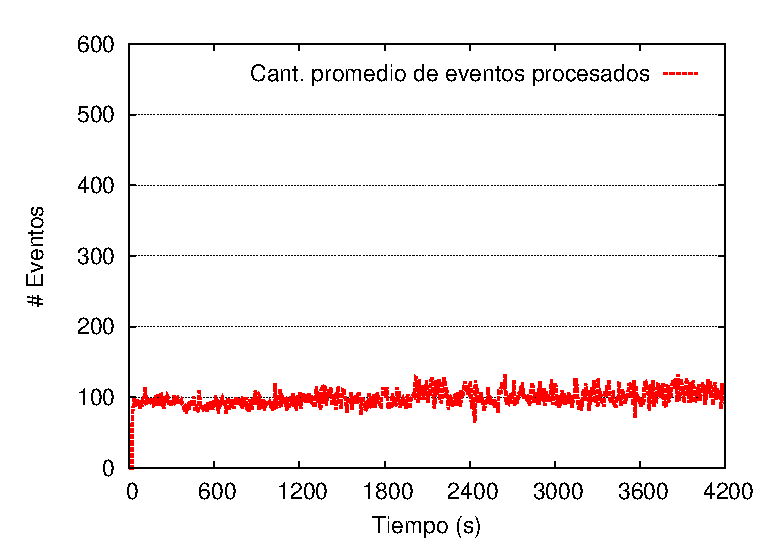
\includegraphics[width=\textwidth]{images/exp/app1/normal/sm/avgEventProcess.eps}
    \caption{Cantidad promedio de eventos procesados en cada período en la primera aplicación con un envío variable de la fuente de datos no usando monitor.}
    \label{fig:app1-normal-sm-avgEventProcess}
\end{minipage}

\end{figure}

\begin{figure}[ht]
\centering

\begin{minipage}[c]{0.45\textwidth}
\centering
    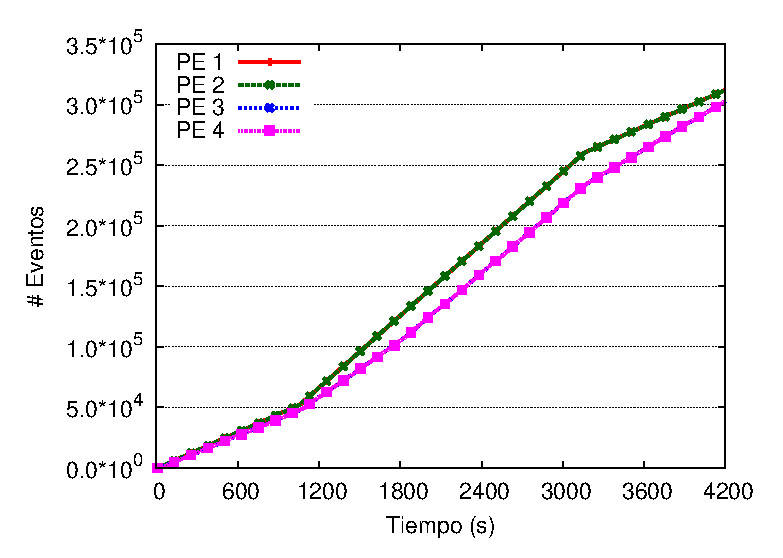
\includegraphics[width=\textwidth]{images/exp/app1/normal/cm/eventCount.eps}
    \caption{Cantidad total de eventos procesados en la primera aplicación con un envío variable de la fuente de datos usando monitor.}
    \label{fig:app1-normal-eventCount-cm}
\end{minipage} \hspace*{1cm}
\begin{minipage}[c]{0.45\textwidth}
\centering
    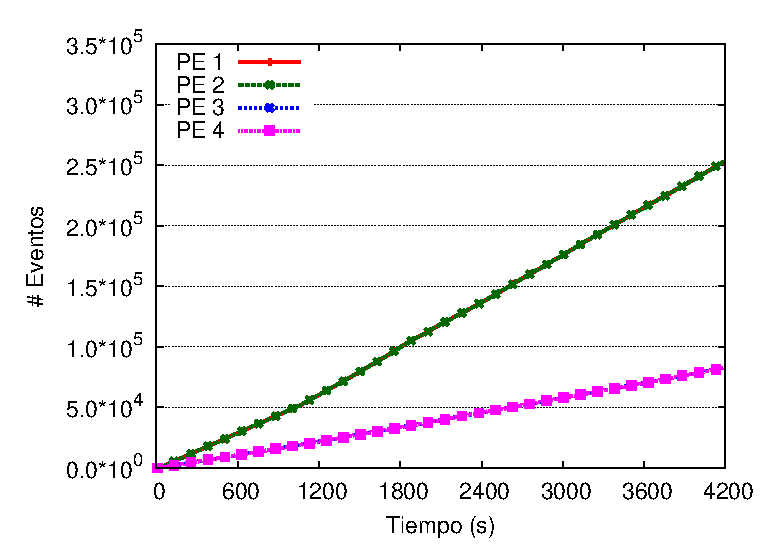
\includegraphics[width=\textwidth]{images/exp/app1/normal/sm/eventCount.eps}
    \caption{Cantidad total de eventos procesados en la primera aplicación con un envío variable de la fuente de datos no usando monitor.}
    \label{fig:app1-normal-eventCount-sm}
\end{minipage}

\end{figure}

\subsection{Aplicación 2: Contador de palabras en muestras de textos}
En la segunda aplicación se procedió a realizar dos experimentos, los cuales eran similares al anterior, donde el primero consta un envío constantes, y el segundo un envío variable. En ambos experimentos, se consideraron dos pruebas, donde la primera consistía en la ejecución de la aplicación en un sistema SPS que use el sistema de distribución de carga, y la segunda sin uso de éste, por lo que cada par de figuras es la comparación de la aplicación con y sin monitor respectivamente.

Para ambos experimentos, se consideró la cantidad total de eventos y las estadísticas de cada PE en el transcurso de la ejecución de la aplicación.

Para analizar el comportamiento del sistema con flujo constante de la fuente de datos, se puede observar en las Figuras \ref{fig:app2-uniform-statusSplitPE-cm} y \ref{fig:app2-uniform-statusSplitPE-sm} las estadísticas del primer operador del grafo, con y sin monitoreo en la carga de los operadores respectivamente. En el primer gráfico la tasa de llegada ($\lambda$) en los primeros 200 segundos se encuentran ciertos \textit{peak}, los cuales se deben al retraso en la toma de estadísticas, producto de la replicación del siguiente PE en el sistema, como se puede demostrar en la Figura \ref{fig:app2-uniform-statusCounterPE-cm}. Independiente del uso del monitor, se puede denotar que el comportamiento entre los dos PEs es prácticamente igual, y eso se debe a la carga que posee el PE es baja. Esto se debe a que este operador es auxiliar, dado que al ser PE Counter un operador con estado, necesita un operador predecesor que separe la cantidad de palabras del \textit{tweets}, de tal manera que el PE Counter cuenta la frecuencia de cada palabra en la información entrante.

En cambio, en las Figuras \ref{fig:app2-uniform-statusCounterPE-cm} y \ref{fig:app2-uniform-statusCounterPE-sm} se puede observar una diferencia en los rendimientos del PE. Esto se debe, a que este operador posee una carga una alta carga, dado que posee una gran bolsa de palabras para comparar con las palabras del \textit{tweets}. Debido a esto, al generar las réplicas, se produce una mejora considerable del operador en los primeros 100 segundo.

En este caso, el predictor se activó, dado que se realiza un aumento de 9 a 14 réplicas. Si bien, la cantidad de réplicas fue mayor a lo necesario, dado que el promedio de tasa de procesamiento posterior al segundo 100 es de 0.63, no se considera el operador en estado ocioso, por lo que no se disminuye la cantidad de réplicas.

Una análisis importante a destacar, es que independiente que el PE Counter se creen más réplicas, el sistema no procesa todos los eventos que van llegando. Esto se puede observar en la cola que existe en el operador, donde se puede apreciar un aumento de ésta con el transcurso del tiempo. Si bien se genera colas igualmente en el sistema con monitoreo, la diferencia que posee con el sistema sin monitoreo es del doble de eventos encolados. Este problema fue detectado por la implementación realizada en S4, debido que los PEs no procesan la cantidad de eventos que deberían en ese período de tiempo. Esto no significa que se pierden datos, simplemente que en caso de no procesarlos, los deja en cola para posteriormente procesarlos. En caso que no se enviaran más datos de la fuente de datos, los eventos en cola se procesan hasta vaciar el \textit{buffer}.

En el último PE, se puede ver que existe una baja cantidad de eventos entrantes, como se muestra en las Figuras \ref{fig:app2-uniform-statusMergePE-cm} y \ref{fig:app2-uniform-statusMergePE-sm}, debido a su condición de PE auxiliar. Cabe recordar que se denomina operador auxiliar a los PEs predecesor y sucesores del posible operador sobrecargado, de esta manera, estos operadores se dedican a dividir la información para enviarla a las distintas réplicas del operador, y posteriormente juntar la información obtenida por las distintas réplicas de éste. La baja cantidad de eventos entrantes se debe a que los eventos entrantes sólo son enviados cada 10 segundos por el PE Counter, por lo que son una pequeña cantidad de eventos los que son enviados. En el primer gráfico, se puede ver que la tasa de llegada aumenta posterior a los 100 segundos, esto se debe a que se realizaron réplicas, por lo que cada una de las réplicas envía un evento cada 10 segundos, habiendo mayor flujo. En cambio, en el segundo gráfico, el flujo de entrada sólo se condiciona por una réplica, por lo que no se procesa la misma cantidad de eventos. Cabe destacar, que como la tasa de llegada es pequeña, no existe un problema en la tasa de rendimiento del operador, aunque posea un alto cómputo de ejecución su tarea.

Finalmente, en las Figuras \ref{fig:app2-uniform-eventCount-cm} y \ref{fig:app2-uniform-eventCount-sm} se muestra la cantidad total de eventos procesados. En el primer gráfico se puede analizar que la diferencia de la pendiente entre las rectas del primer y segundo PE, es menor que en el segundo gráfico. Esto se debe al aumento de la cantidad de réplicas, de esta manera puede procesar mayor cantidad de eventos, siendo un procesamiento de 275.290 con uso el monitor contra 28.152 sin uso del monitor, habiendo una mejora de 8 veces más eventos. El tercer PE procesa pocos eventos, debido que sólo le llega un evento por réplica cada 10 segundos.

Dentro de los análisis importantes a realizar por parte de este experimento, es que en la Figura \ref{fig:app2-uniform-eventCount-cm} no existe una mejora por parte del segundo PE de manera paralela al flujo de datos emanado por el primer PE. Como se había explicado anteriormente, independiente que se generen más réplicas, los operadores igualmente va a encolar cierta cantidad de eventos, debido a la implementación de S4.

\begin{figure}[p]
\centering
    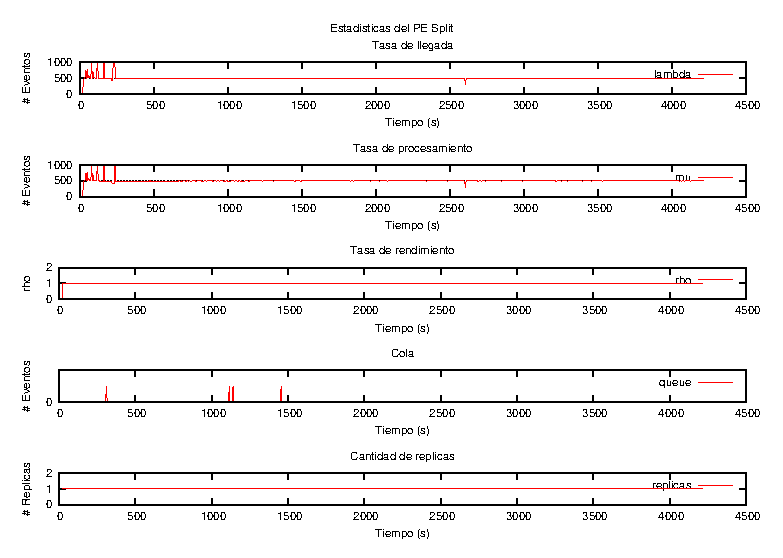
\includegraphics[scale=1.1]{images/exp/app2/uniform/cm/statusSplitPE.eps}
    \caption{Estadísticas del PE Split en la segunda aplicación con un envío constante de la fuente de datos con uso del monitor.}
    \label{fig:app2-uniform-statusSplitPE-cm}
\end{figure}

\begin{figure}[p]
\centering
    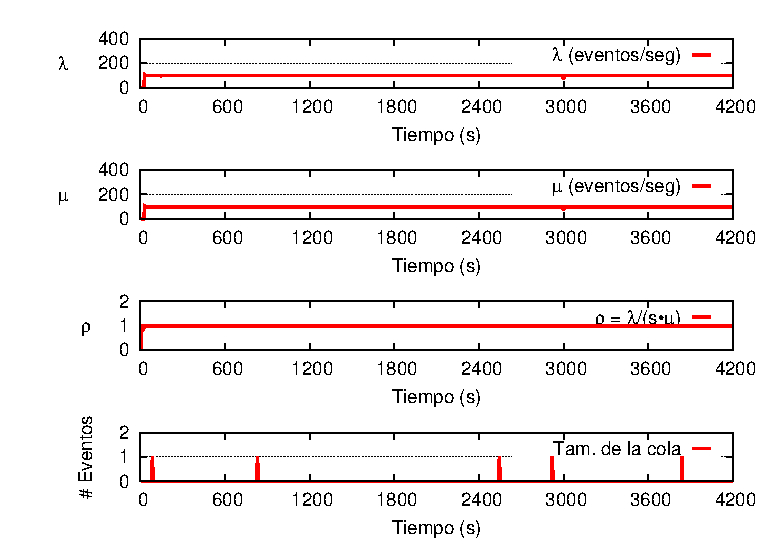
\includegraphics[scale=1.1]{images/exp/app2/uniform/sm/statusSplitPE.eps}
    \caption{Estadísticas del PE Split en la segunda aplicación con un envío constante de la fuente de datos sin uso del monitor.}
    \label{fig:app2-uniform-statusSplitPE-sm}
\end{figure}

\begin{figure}[p]
\centering
    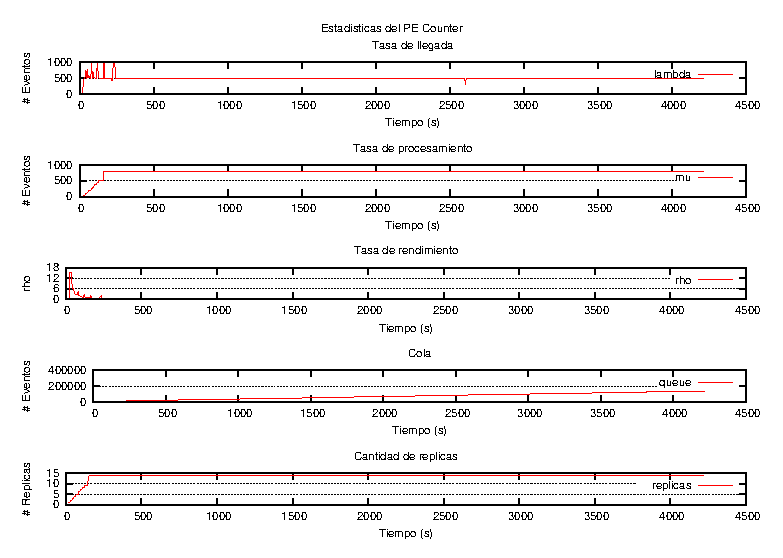
\includegraphics[scale=1.1]{images/exp/app2/uniform/cm/statusCounterPE.eps}
    \caption{Estadísticas del PE Counter en la segunda aplicación con un envío constante de la fuente de datos con uso del monitor.}
    \label{fig:app2-uniform-statusCounterPE-cm}
\end{figure}

\begin{figure}[p]
\centering
    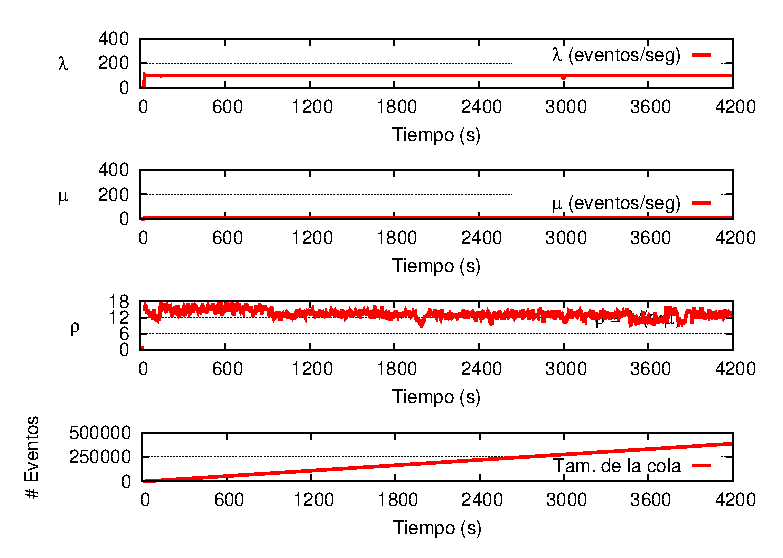
\includegraphics[scale=1.1]{images/exp/app2/uniform/sm/statusCounterPE.eps}
    \caption{Estadísticas del PE Counter en la segunda aplicación con un envío constante de la fuente de datos sin uso del monitor.}
    \label{fig:app2-uniform-statusCounterPE-sm}
\end{figure}

\begin{figure}[p]
\centering
    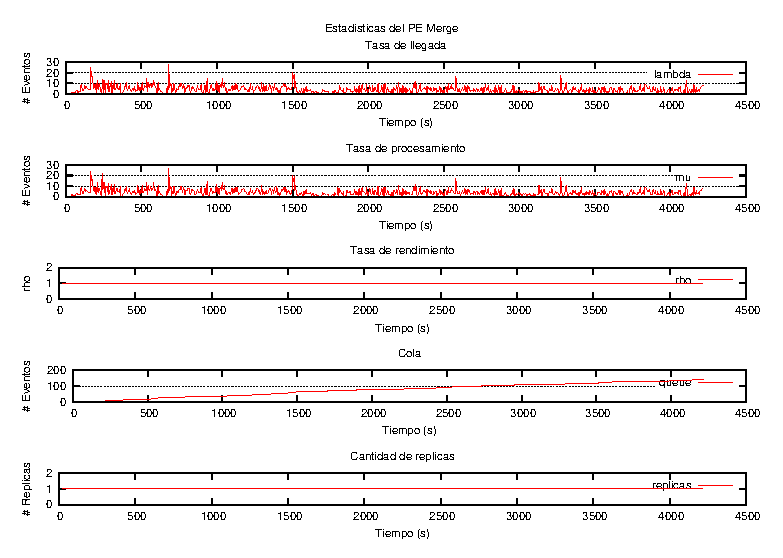
\includegraphics[scale=1.1]{images/exp/app2/uniform/cm/statusMergePE.eps}
    \caption{Estadísticas del PE Merge en la segunda aplicación con un envío constante de la fuente de datos con uso del monitor.}
    \label{fig:app2-uniform-statusMergePE-cm}
\end{figure}

\begin{figure}[p]
\centering
    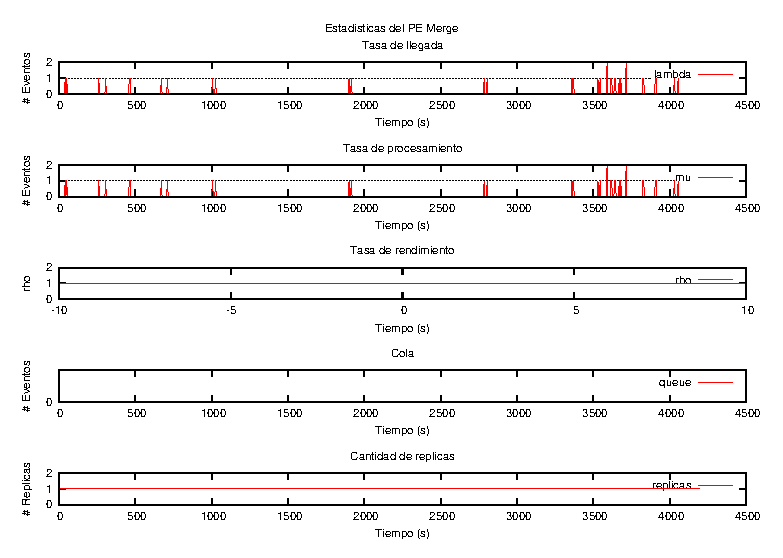
\includegraphics[scale=1.1]{images/exp/app2/uniform/sm/statusMergePE.eps}
    \caption{Estadísticas del PE Merge en la segunda aplicación con un envío constante de la fuente de datos sin uso del monitor.}
    \label{fig:app2-uniform-statusMergePE-sm}
\end{figure}

\begin{figure}[ht]
\centering

\begin{minipage}[c]{0.45\textwidth}
\centering
    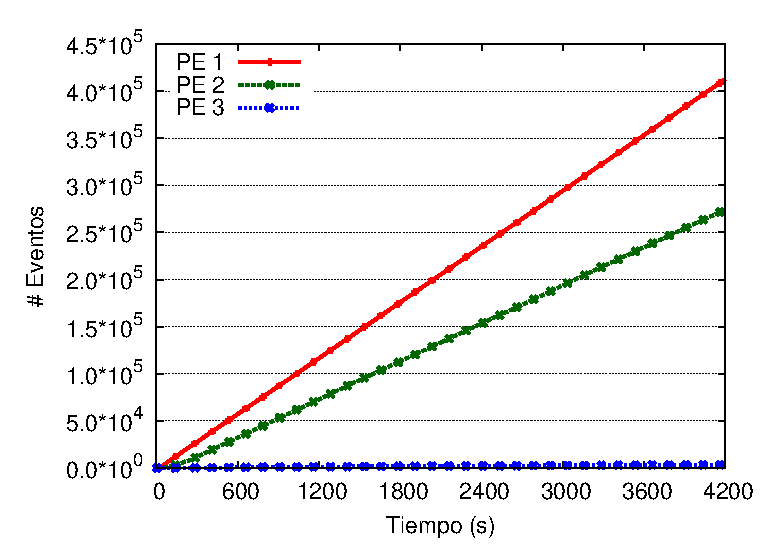
\includegraphics[width=\textwidth]{images/exp/app2/uniform/cm/eventCount.eps}
    \caption{Cantidad total de eventos procesados en la segunda aplicación con un envío constante de la fuente de datos no usando usando monitor.}
    \label{fig:app2-uniform-eventCount-cm}
\end{minipage} \hspace*{1cm}
\begin{minipage}[c]{0.45\textwidth}
\centering
    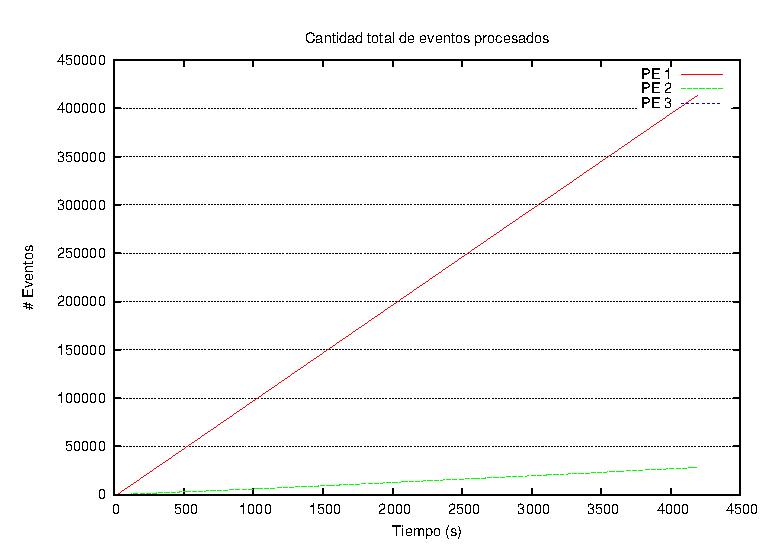
\includegraphics[width=\textwidth]{images/exp/app2/uniform/sm/eventCount.eps}
    \caption{Cantidad total de eventos procesados en la segunda aplicación con un envío constante de la fuente de datos no usando no usando monitor.}
    \label{fig:app2-uniform-eventCount-sm}
\end{minipage}

\end{figure}

Para analizar el comportamiento del sistema con flujo variable de la fuente de datos, se puede observar en las Figuras \ref{fig:app2-normal-statusSplitPE-cm} y \ref{fig:app2-normal-statusSplitPE-sm} las estadísticas del primer operador del grafo, con y sin monitoreo en la carga de los operadores respectivamente. Como se había explicado en el primer experimento, en las estadísticas con monitor se puede ver ciertos \textit{peaks}, los cuales son provocados por el sistema de monitoreo existente. Aunque estos sean representados gráficamente, no presentan un problema a la hora de realizar una análisis del sistema por parte del sistema de monitoreo en este experimento. Debido que el PE posee un bajo nivel de cómputo, dada la tarea que realiza, no existe una tasa de rendimiento que sea inestable, tanto para el sistema con y sin uso del monitoreo, por lo que no existen mayores problemas en éste.

A diferencia del anterior PE, en el segundo PE si existe un nivel de sobrecarga importante, como se puede apreciar en las Figuras \ref{fig:app2-normal-statusCounterPE-cm} y \ref{fig:app2-normal-statusCounterPE-sm}. En los primeros 100 segundos existe una inestabilidad en el sistema, el cual se estabiliza en posteriormente en el sistema con uso del monitor, dado que réplica el operador. Esta inestabilidad se vuelve apreciar en el segundo 1100, cuando aumenta el envío de datos desde la fuente de datos, lo cual hace que la cantidad de réplicas existentes sean insuficientes, por lo que el sistema debe volver a replicar. Para que en el último tramo, en el segundo 3200 disminuya la cantidad de réplicas, debido que el envío de datos disminuyó por parte de la fuente de datos.

Como se había explicado en el mismo experimento de envío variable de la fuente de datos en la aplicación 1, la cantidad óptima de operadores en el primer tramo es distinta a la del tercer tramo. Esto se debe a que en el primer tramo van aumentando la cantidad de réplicas para ir convergiendo $\rho$ a un valor de 1, en cambio, en el tercer tramo se va disminuye la cantidad de réplicas para ir convergiendo $\rho$ a 0.5, límite inferior para definir el estado estable.

Otro dato importante a analizar, es que en este experimento no se activó el predictor, y esto se debe a que la replicación fue paulatina, por lo que alcanzó a generar una convergencia de la cantidad de operadores necesarios antes que el predictor pudiera detectar que existe una inestabilidad en el operador.

En el tercer PE, se puede analizar que la tasa de llegada es baja tanto en las Figuras \ref{fig:app2-normal-statusMergePE-cm} y \ref{fig:app2-normal-statusMergePE-sm}, y esto se debe a que este PE es auxiliar como se explicó anteriormente, por lo que sólo le llegan eventos de los emitidos por cada PE Counter en un período de tiempo dado. El análisis que se realiza en el PE Merge es el mismo explicado en el anterior experimento, donde la tasa de llegada va a depender de la cantidad de réplicas existentes en el PE Counter, por lo que la tasa de llegada es mayor en el sistema con monitoreo.

Finalmente, en las Figuras \ref{fig:app2-uniform-eventCount-cm} y \ref{fig:app2-uniform-eventCount-sm} se muestra la cantidad total de eventos procesados. En el primer gráfico se puede apreciar que la curva del primer PE y el segundo PE es más cercana que las que se observan en el segundo gráfico, y esto se debe a la replicación que efectúo el sistema. Cabe destacar que el sistema utilizando el monitor proceso un total de $228.942$ eventos, mientras que la version sin monitor solo alcanzo a procesar $27.751$ eventos. Por lo que nuestra solución permitió aumentar en más de 8 veces la cantidad de eventos procesados.

\begin{figure}[p]
\centering
    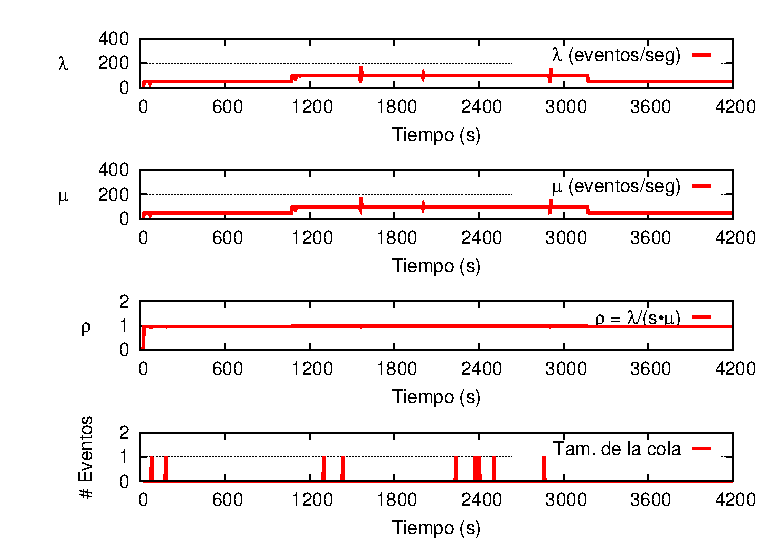
\includegraphics[scale=1.1]{images/exp/app2/normal/cm/statusSplitPE.eps}
    \caption{Estadísticas del PE Split en la segunda aplicación con un envío variable de la fuente de datos con uso del monitor.}
    \label{fig:app2-normal-statusSplitPE-cm}
\end{figure}

\begin{figure}[p]
\centering
    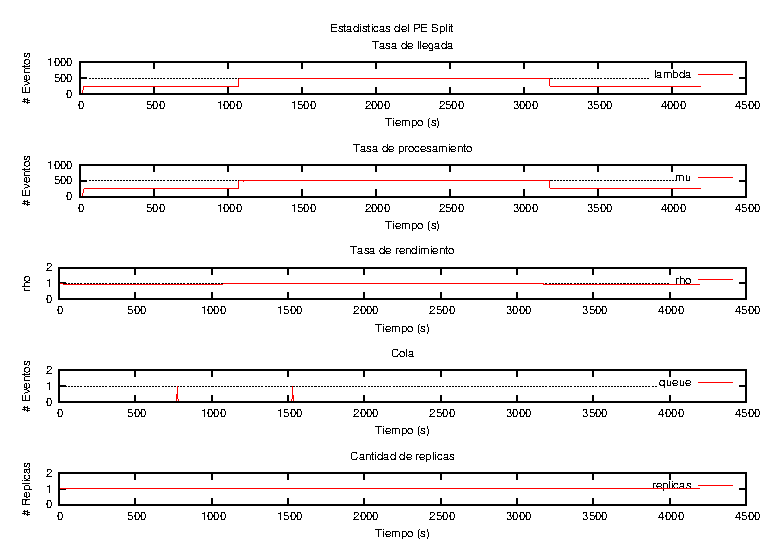
\includegraphics[scale=1.1]{images/exp/app2/normal/sm/statusSplitPE.eps}
    \caption{Estadísticas del PE Split en la segunda aplicación con un envío variable de la fuente de datos sin uso del monitor.}
    \label{fig:app2-normal-statusSplitPE-sm}
\end{figure}

\begin{figure}[p]
\centering
    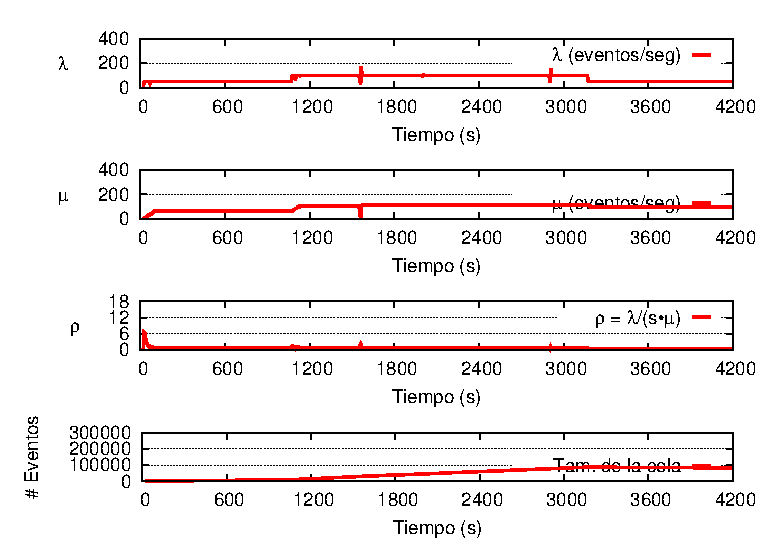
\includegraphics[scale=1.1]{images/exp/app2/normal/cm/statusCounterPE.eps}
    \caption{Estadísticas del PE Counter en la segunda aplicación con un envío variable de la fuente de datos con uso del monitor.}
    \label{fig:app2-normal-statusCounterPE-cm}
\end{figure}

\begin{figure}[p]
\centering
    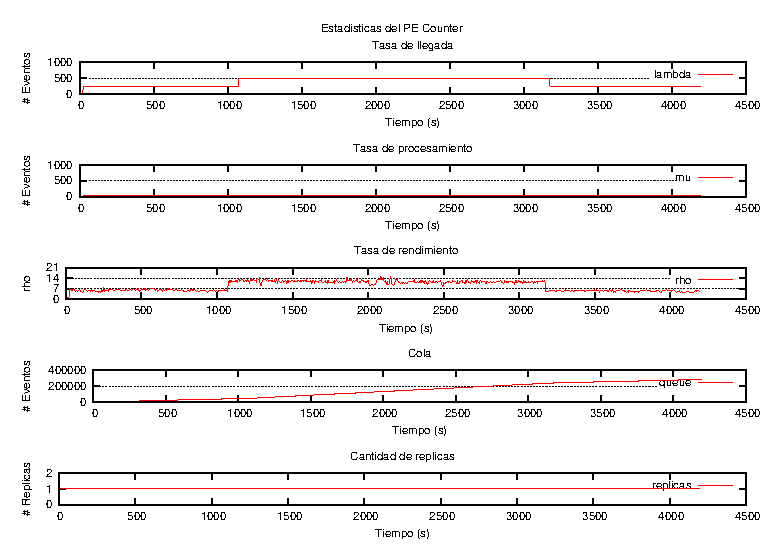
\includegraphics[scale=1.1]{images/exp/app2/normal/sm/statusCounterPE.eps}
    \caption{Estadísticas del PE Counter en la segunda aplicación con un envío variable de la fuente de datos sin uso del monitor.}
    \label{fig:app2-normal-statusCounterPE-sm}
\end{figure}

\begin{figure}[p]
\centering
    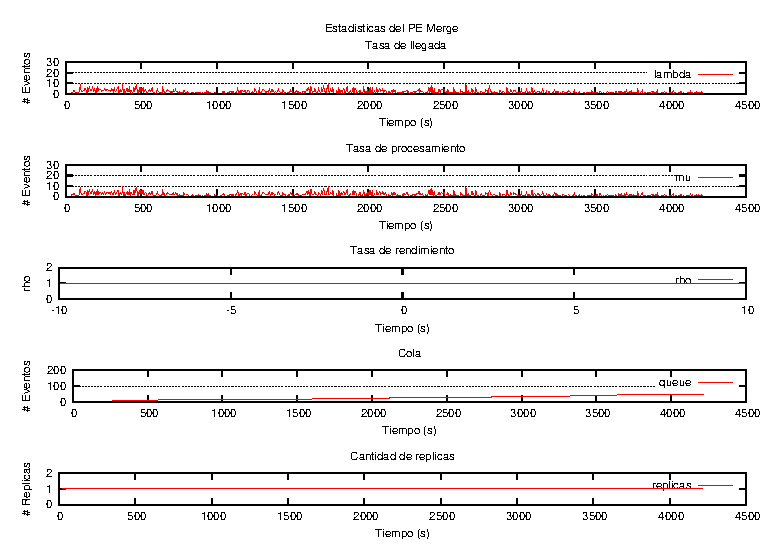
\includegraphics[scale=1.1]{images/exp/app2/normal/cm/statusMergePE.eps}
    \caption{Estadísticas del PE Merge en la segunda aplicación con un envío variable de la fuente de datos con uso del monitor.}
    \label{fig:app2-normal-statusMergePE-cm}
\end{figure}

\begin{figure}[p]
\centering
    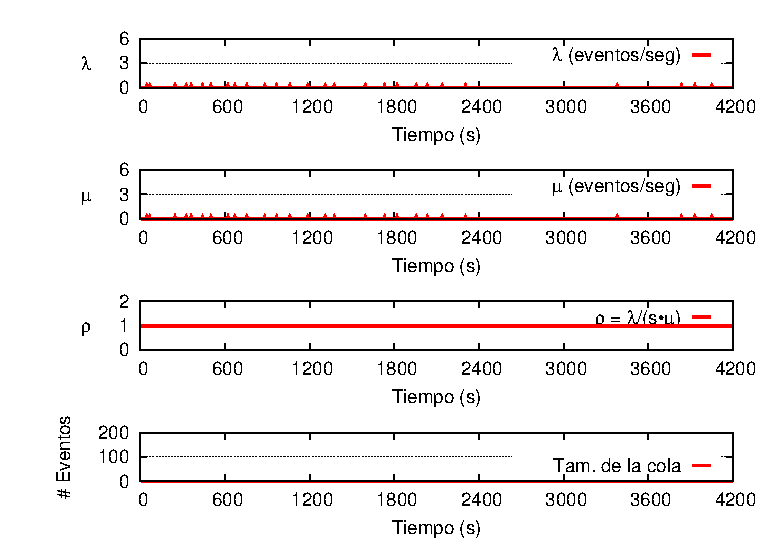
\includegraphics[scale=1.1]{images/exp/app2/normal/sm/statusMergePE.eps}
    \caption{Estadísticas del PE Merge en la segunda aplicación con un envío variable de la fuente de datos sin uso del monitor.}
    \label{fig:app2-normal-statusMergePE-sm}
\end{figure}

\begin{figure}[ht]
\centering

\begin{minipage}[c]{0.45\textwidth}
\centering
    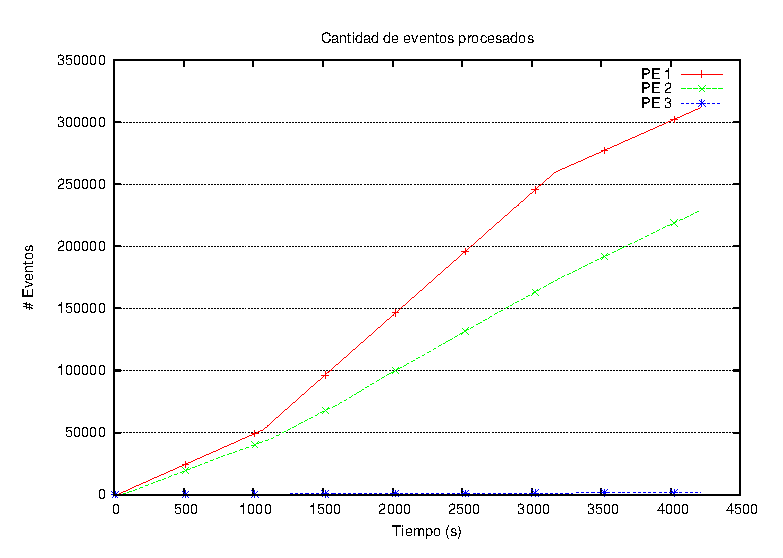
\includegraphics[width=\textwidth]{images/exp/app2/normal/cm/eventCount.eps}
    \caption{Cantidad total de eventos procesados en la segunda aplicación con un envío variable de la fuente de datos usando monitor.}
    \label{fig:app2-normal-eventCount-cm}
\end{minipage} \hspace*{1cm}
\begin{minipage}[c]{0.45\textwidth}
\centering
    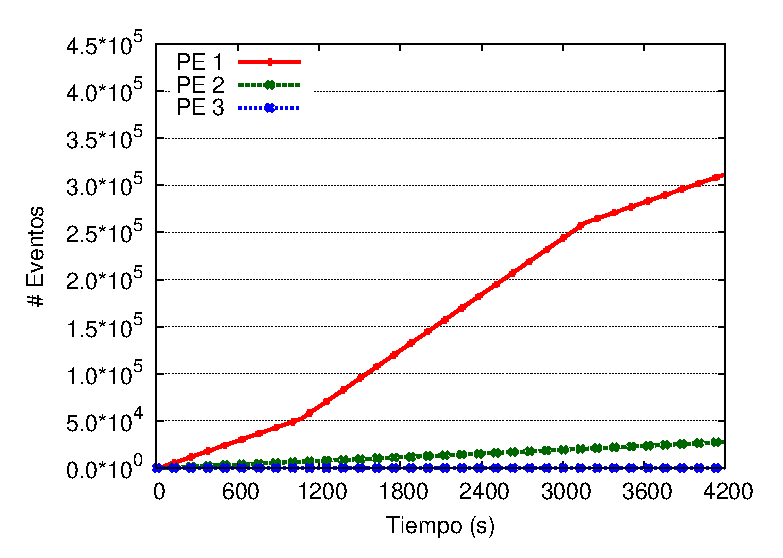
\includegraphics[width=\textwidth]{images/exp/app2/normal/sm/eventCount.eps}
    \caption{Cantidad total de eventos procesados en la segunda aplicación con un envío variable de la fuente de datos no usando monitor.}
    \label{fig:app2-normal-eventCount-sm}
\end{minipage}

\end{figure}

\subsection{Aplicación 3: Aplicación sintética}
En la tercera aplicación se procedió a realizar dos experimentos, ambos con envío constante de 100 eventos por segundo de la fuente de datos, donde el SPS funciona con y sin uso del monitor.

Para el análisis de los experimentos se consideró el consumo de RAM, el uso de la CPU, la cantidad total de eventos y las estadísticas de cada PE en el transcurso de la ejecución de la aplicación.

Respecto a la utilización de CPU, se puede observar en las Figuras \ref{fig:app3-consumeCPU-cm} y \ref{fig:app3-consumeCPU-sm} el porcentaje de uso con y sin monitoreo. En el primer caso existe un $0.621\%$ de utilización de CPU, contra un $0.6091\%$ del segundo caso, habiendo un aumento del $0,0119\%$ de utilización promedio de CPU. Dentro de los primeros 10 segundo existe un alto uso de CPU en ambos gráficos, y eso se debe que es el \textit{deploy} y compilación de la aplicación en el sistema de S4.

Por otra parte, el consumo de memoria RAM está dado por las Figuras \ref{fig:app3-consumeRAM-cm} y \ref{fig:app3-consumeRAM-sm}, donde la primera es con uso de monitoreo y la segundo no. En el primer gráfico existe un consumo promedio de $264,8033$ MB, contra $268,8667$ MB del segundo gráfico, habiendo una disminución del $1,5187\%$ de consumo de memoria RAM. En el primer gráfico se puede observar un aumento del consumo de memoria en el segundo 200, a diferencia del segundo gráfico, y esto se debe a que al consumir mayor cantidad de eventos y generar nuevos operadores, existe un mayor consumo de memoria por parte del sistema. Pero posterior al segundo 600, por parte del sistema sin monitoreo, se muestra un aumento del consumo de memoria, lo cual se debe a la cantidad de eventos en cola que existen en el sistema, a diferencia del primer gráfico que hubo una convergencia en el consumo de la memoria, por lo que posteriormente el reducir las colas, reduce igualmente el consumo de memoria RAM en la ejecución.

En cuanto a la cantidad total de eventos procesados, en las Figuras \ref{fig:app3-eventCount-cm} y \ref{fig:app3-eventCount-sm} se puede apreciar que la cantidad de eventos procesados es mayor en el gráfico con uso del monitor. En el primer gráfico existe un total de $88.169$ eventos procesados y en el segundo un total de $29.714$ eventos procesados, existiendo una mejora de 3 veces la cantidad de eventos procesados

Finalmente, en las Figuras \ref{fig:app3-statusOnePE-cm} y \ref{fig:app3-statusOnePE-sm} se presentan las estadísticas del primer PE, el cual se muestra una diferencia en la tasa de procesamiento en los experimentos con y sin monitor, lo cual afecta en la tasa de llegada del segundo PE como muestra las Figura \ref{fig:app3-statusTwoPE-cm} y \ref{fig:app3-statusTwoPE-sm}. Finalmente, en las Figuras \ref{fig:app3-statusThreePE-cm} y \ref{fig:app3-statusThreePE-sm} se presenta el tercer PE, en el cual no existe variación en su tasa de rendimiento en ninguno de los dos casos, debido que en el experimento sin monitoreo recibe una menor tasa de llegada, dada la tasa de procesamiento del PE anterior.

\begin{figure}[!hptb]
\centering

\begin{minipage}[c]{0.45\textwidth}
\centering
    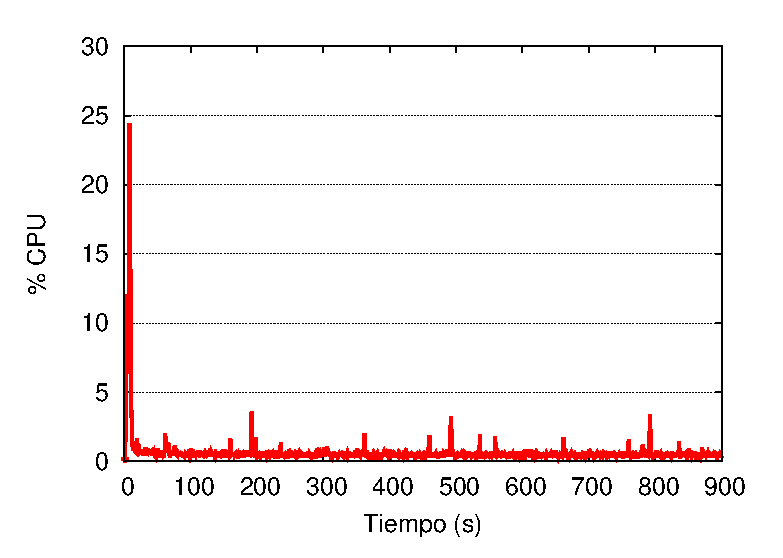
\includegraphics[width=\textwidth]{images/exp/app3/cm/fisical/consumeCPU.eps}
    \caption{Porcentaje de utilización de la CPU en la tercera aplicación usando monitor.}
    \label{fig:app3-consumeCPU-cm}
\end{minipage} \hspace*{1cm}
\begin{minipage}[c]{0.45\textwidth}
\centering
    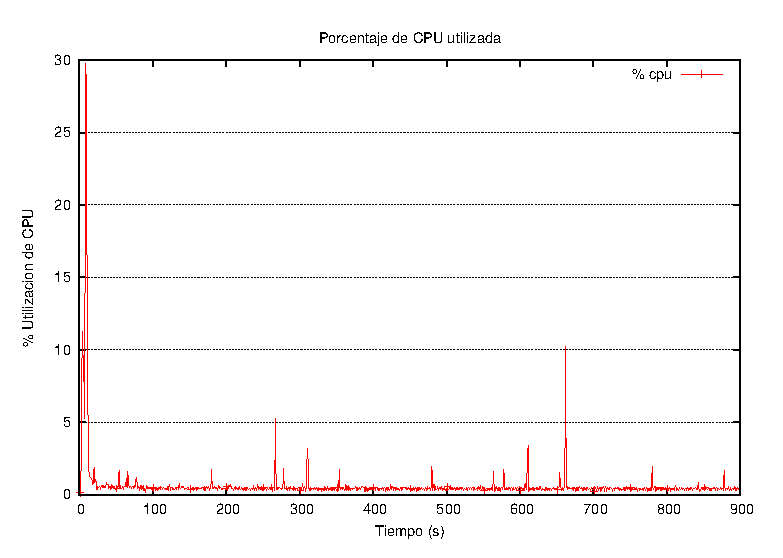
\includegraphics[width=\textwidth]{images/exp/app3/sm/fisical/consumeCPU.eps}
    \caption{Porcentaje de utilización de la CPU en la tercera aplicación no usando monitor.}
    \label{fig:app3-consumeCPU-sm}
\end{minipage}

\end{figure}

\begin{figure}[!hptb]
\centering

\begin{minipage}[c]{0.45\textwidth}
\centering
    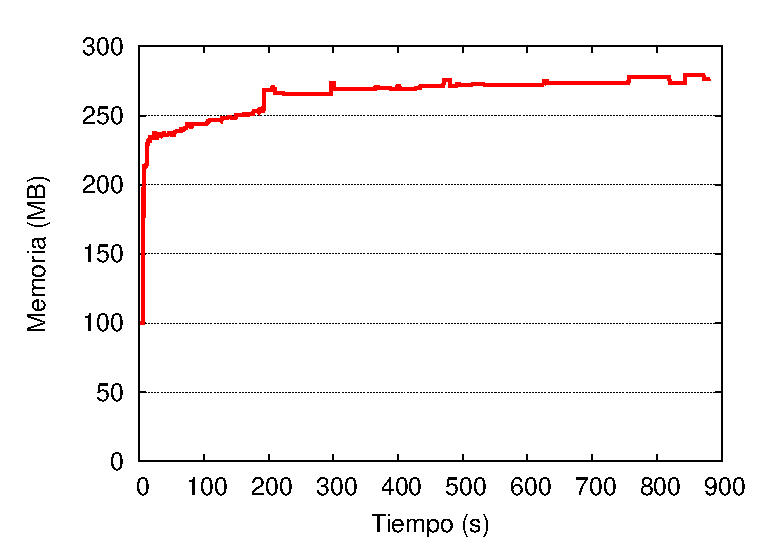
\includegraphics[width=\textwidth]{images/exp/app3/cm/fisical/consumeRAM.eps}
    \caption{Consumo de memoria RAM en la tercera aplicación usando monitor.}
    \label{fig:app3-consumeRAM-cm}
\end{minipage} \hspace*{1cm}
\begin{minipage}[c]{0.45\textwidth}
\centering
    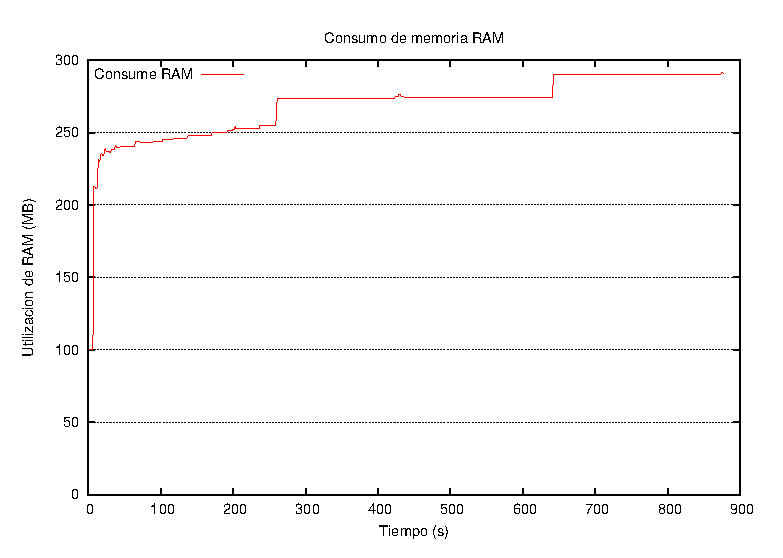
\includegraphics[width=\textwidth]{images/exp/app3/sm/fisical/consumeRAM.eps}
    \caption{Consumo de memoria RAM en la tercera aplicación no usando monitor.}
    \label{fig:app3-consumeRAM-sm}
\end{minipage}

\end{figure}

\begin{figure}[!hptb]
\centering

\begin{minipage}[c]{0.45\textwidth}
\centering
    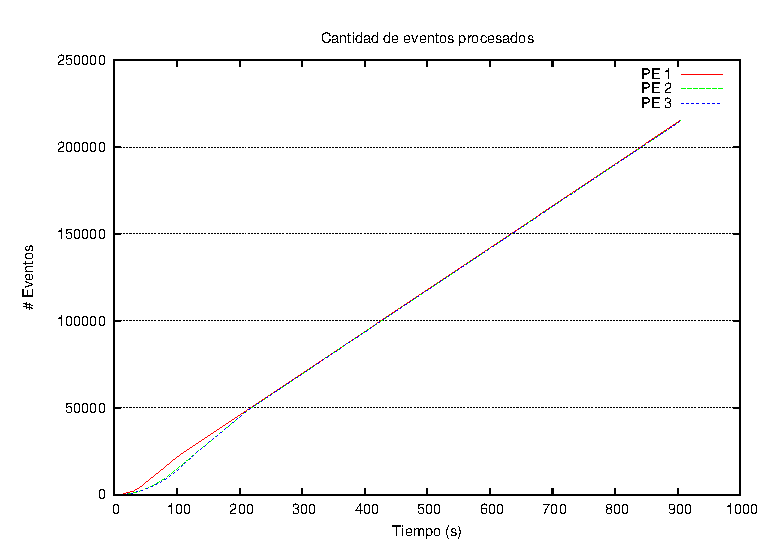
\includegraphics[width=\textwidth]{images/exp/app3/cm/logical/eventCount.eps}
    \caption{Cantidad de eventos procesados en la tercera aplicación usando monitor.}
    \label{fig:app3-eventCount-cm}
\end{minipage} \hspace*{1cm}
\begin{minipage}[c]{0.45\textwidth}
\centering
    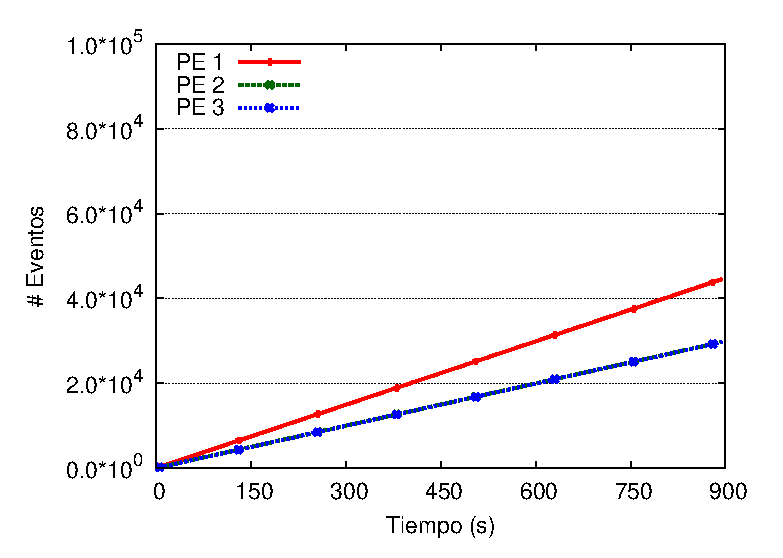
\includegraphics[width=\textwidth]{images/exp/app3/sm/logical/eventCount.eps}
    \caption{Cantidad de eventos procesados en la tercera aplicación no usando monitor.}
    \label{fig:app3-eventCount-sm}
\end{minipage}

\end{figure}

\begin{figure}[!hptb]
\centering
    \includegraphics[scale=1.1]{images/exp/app3/cm/logical/statusOnePE.eps}
    \caption{Estadísticas del primer PE en la tercera aplicación con un envío constante de la fuente de datos con uso del monitor.}
    \label{fig:app3-statusOnePE-cm}
\end{figure}

\begin{figure}[!hptb]
\centering
    \includegraphics[scale=1.1]{images/exp/app3/sm/logical/statusOnePE.eps}
    \caption{Estadísticas del primer PE en la tercera aplicación con un envío constante de la fuente de datos sin uso del monitor.}
    \label{fig:app3-statusOnePE-sm}
\end{figure}

\begin{figure}[!hptb]
\centering
  uniform  \includegraphics[scale=1.1]{images/exp/app3/cm/logical/statusTwoPE.eps}
    \caption{Estadísticas del segundo PE en la tercera aplicación con un envío constante de la fuente de datos con uso del monitor.}
    \label{fig:app3-statusTwoPE-cm}
\end{figure}

\begin{figure}[!hptb]
\centering
    \includegraphics[scale=1.1]{images/exp/app3/sm/logical/statusTwoPE.eps}
    \caption{Estadísticas del segundo PE en la tercera aplicación con un envío constante de la fuente de datos sin uso del monitor.}
    \label{fig:app3-statusTwoPE-sm}
\end{figure}

\begin{figure}[!hptb]
\centering
    \includegraphics[scale=1.1]{images/exp/app3/cm/logical/statusThreePE.eps}
    \caption{Estadísticas del tercer PE en la tercera aplicación con un envío constante de la fuente de datos con uso del monitor.}
    \label{fig:app3-statusThreePE-cm}
\end{figure}

\begin{figure}[!hptb]
\centering
    \includegraphics[scale=1.1]{images/exp/app3/sm/logical/statusThreePE.eps}
    \caption{Estadísticas del tercer PE en la tercera aplicación con un envío constante de la fuente de datos sin uso del monitor.}
    \label{fig:app3-statusThreePE-sm}
\end{figure}

\vspace*{15cm}